\documentclass[a4paper,10pt]{article}
\pdfoutput=1 % if your are submitting a pdflatex (i.e. if you have
             % images in pdf, png or jpg format)
\usepackage{jcappub} % for details on the use of the package, please
                     % see the JCAP-author-manual          
\usepackage{enumitem}% http://ctan.org/pkg/enumitem
\usepackage[T1]{fontenc} % if needed
\usepackage{hyperref}

\graphicspath{ {images/} }


\renewcommand{\v}[1]{\mathbf{#1}}
\newcommand{\Mp}{M_{pl}}
\newcommand{\half}{\frac{1}{2}}
\newcommand{\bphi}{\bar{\phi}}
\newcommand{\ann}[1]{\hat{a}_{\v{#1}}}
\newcommand{\cre}[1]{\hat{a}^\dagger_{\v{#1}}}
\newcommand{\anns}[2]{\hat{a}_{\v{#1}#2}}
\newcommand{\cres}[2]{\hat{a}^\dagger_{\v{#1}#2}}
\newcommand{\vac}{|0\rangle}
\newcommand{\fint}[1]{\int \frac{d^3 \v{#1}}{(2\pi)^3}}
\newcommand{\finttwo}[1]{\int \frac{d^2 \v{#1}}{(2\pi)^2}}
\newcommand{\unit}[1]{\hat{\v{#1}}}
\newcommand{\sr}{\text{\normalfont\dh}}
\renewcommand{\sl}{\bar{\text{\normalfont\dh}}}
\newcommand{\ltwo}{[\frac{(l+2)!}{(l-2)!}]}
\newcommand{\ltwof}{[\frac{(l-2)!}{(l+2)!}]}

\title{\boldmath The Search for CMB B-mode Polarization from Inflationary Gravitational Waves}


%% %simple case: 2 authors, same institution
%% \author{A. Uthor}
%% \author{and A. Nother Author}
%% \affiliation{Institution,\\Address, Country}

% more complex case: 4 authors, 3 institutions, 2 footnotes
\author{B. Chughtai}

% The "\note" macro will give a warning: "Ignoring empty anchor..."
% you can safely ignore it.

\affiliation{University of Cambridge, Cambridge, UK}


% e-mail addresses: one for each author, in the same order as the authors
\emailAdd{bc464@cam.ac.uk}




\abstract{Abstract...}



\begin{document}
\maketitle
\flushbottom


\section{Introduction}

define scale factor
define conformal time
define dot and '
units hbar = c = 1
fourier convention

\section{Inflationary Cosmology}
\nocite{*}
\cite{QBM}

Inflation is a brief, but very important, period of accelerated expansion in the very early universe, first proposed by [Guth 1981]. It was initially motivated by three problems with the previous standard big bang cosmology, namely the flatness problem (why was the ratio of energy density and critical density so close to unity), the monopole problem, and the horizon problem (why are seemingly casually disconnected regions of the CMB at the same temperature to very high accuracy). Since the birth of the idea, it has become the leading paradigm to the early universe, in part because it provides a quantum mechanical mechanism of generating the primordial density perturbations seeding cosmological evolution. In this chapter we quickly review some important features of inflation.

\subsection{Inflation Basics}

A flat, homogeneous and isotropic universe is described by the Friedmann–Lemaître–Robertson–Walker (FLRW) metric, which in our sign convention takes form

\begin{equation}
\label{FLRW}
ds^2 = - dt^2 + a^2(t)d\v{x}^2 = a^2(\tau)(-d\tau^2+d\v{x}^2)
\end{equation}

and, assuming General Relativity, obeys the Einstein equation $G_{ab} = \frac{1}{\Mp^2} T_{ab}$, sourced by a perfect fluid with energy momentum tensor $T_{ab}$, which by homogeneity and isotropy must take form

\begin{equation}
\label{densityandpressure}
T^0_0 = - \rho(t) \quad T^0_i = 0 \quad T^i_j = P(t)\delta^i_j
\end{equation}

where we  identify $\rho(t)$ as the total energy density and $P(t)$ as the total pressure. For our purposes, we will consider one component, the inflaton field, to dominate.  Substituting \ref{FLRW} and \ref{densityandpressure} into the Einstein Equation we obtain the Friedmann equations

\begin{equation}
H^2 = (\frac{\dot{a}}{a})^2 = \frac{1}{3\Mp^2}\rho
\tag{F1}
\label{F1}
\end{equation}
\begin{equation}
\dot{H} + H^2 = \frac{\ddot{a}}{a} = -\frac{1}{6\Mp^2}(\rho + 3P)
\tag{F2}
\label{F2}
\end{equation}

The condition for inflation to occur is \textit{accelerated expansion}, ie $\ddot{a} >0$. Recalling the definition of the first hubble slow roll parameter 

\begin{equation}
\label{epsilon}
\epsilon := -\frac{\dot{H}}{H^2} = -\frac{d\ln{H}}{d\ln{a}} = \frac{3}{2}(1+\frac{P}{\rho})
\end{equation}

,where the last inequality follows from the Friedmann Equations, we find $\ddot{a} >0$ is equivalent to $\epsilon<1$ and to the condition on the equation of state parameter $\omega=P/\rho < -1/3$.\\ 

In order to solve the horizon problem we require inflation to persist for a relatively long duration of time (~60 e-folds), so $\epsilon$ to must remain small. We parametrise how quickly $\epsilon$ changes in the second hubble slow roll parameter 

\begin{equation}
\eta = -\frac{\dot{\epsilon}}{H\epsilon} = -\frac{d\ln{\epsilon}}{d\ln{a}}
\end{equation}

which we also require to be small during inflation.

\subsubsection{Single Scalar Field Dynamics}

The simplest class of inflation models are those consisting of a single scalar field, slowly rolling down its potential. These postulate the existence of a single effective scalar degree of freedom - the ``inflation'' field $\phi(t,\v{x})$ with Lagrangian density $\mathcal{L} = -\half \partial^\mu \phi \partial_\mu \phi - V(\phi)$. Inserting the energy momentum tensor for this lagrangian into \ref{densityandpressure} and the Friedmann equations we obtain the equations of motion for the classical background $\phi(t)$


\begin{equation}\begin{split}
H^2 &= \frac{1}{3\Mp^2}(\half\dot{\phi}^2+V(\phi))\\
\frac{\ddot{a}}{a} &= -\frac{1}{3\Mp^2}(\dot{\phi}^2-V(\phi))\\
\end{split}\end{equation}

and

\begin{equation}
\tag{KG}
\label{KG}
\ddot{\phi}+3H\dot{\phi}=-V_{,\phi}
\end{equation}

From these we see the spacetime axperiences accelerated expansion iff the potential energy dominates the kinetic: $V >> \dot{\phi}^2$ and is sustained if $|\ddot{\phi}| << |V_{,\phi}|$. We also find that by \ref{epsilon} that 

\begin{equation}
\epsilon = \frac{1}{\Mp^2}\frac{\half\dot{\phi}^2}{H^2} < 1
\end{equation}

\subsubsection{Slow Roll}

The slow roll approximation postulates the kinetic energy and acceleration of the background field is much smaller than its potential energy, encapsulated in terms of our slow roll parameters as $(\epsilon, \eta << 1)$. In this approximation we get by \ref{F1} and \ref{KG} 

\begin{equation}\begin{split}
H^2 &\approx \frac{V}{3\Mp^2} \\
3H\dot{\phi} &\approx -V_{,\phi}
\end{split}\end{equation}

from which we see 

\begin{equation}
\epsilon \approx \half\Mp^2 (\frac{V'}{V})^2 := \epsilon_V
\end{equation}

where we have defined the first \textit{potential} slow roll parameter. We can analogously define a second potential slow roll parameter via

\begin{equation}
\eta_V = \Mp^2 \frac{V''}{V} \approx 2\epsilon - \half\eta
\end{equation}

which must therefore also be small. With these constraints satisfied, inflation occurs and inflates the universe in a quasi-deSitter fashion:

\begin{equation}
a(t) \approx a(0)e^{Ht} \qquad H\approx\text{constant}
\end{equation} 
 
For inflation to address the problems with the standard hot big bang we require the number of e-folds to be at least $N_e > \ln{10^{26}} \approx 55$. Since $\phi$ acts as a clock during inflation, we may express the number of e-folds from a time $t$ until the end of inflation as an integral over field excursion instead of time:

\begin{equation}
N(t) := \ln{\frac{a(t_{end})}{a(t)}} = \int_a^{a(t)} d(\ln{a}) = \int_t^{t_{end}} Hdt = \int_{\phi(t)}^{\phi_{end}} \frac{d\phi}{\sqrt{2\epsilon}\Mp}
\label{efolds}
\end{equation}

using $Hdt=\frac{H}{\dot{\phi}}d\bphi=\frac{d\phi}{\sqrt{2\epsilon}\Mp}$


\subsection{Cosmological Perturbation Theory}

Above we only considered the background evolution of the inflaton, though in general it can also vary in space. The metric also experiences perturbations.

\begin{equation}
\phi(t,\v{x}) = \bphi(t) +\delta\phi(t,\v{x}) \qquad g_{\mu\nu}(t,\v{x}) = \bar{g}_{\mu\nu}(t,\v{x})
\end{equation}

where the metric can be written

\begin{equation}
\begin{split}
ds^2 &= g_{\mu\nu}dx^\mu dx^\nu\\
&= -(1+2\Phi)dt^2 + 2aB_idx^idt+a^2[(1-2\Psi)\delta_{ij}+E_{ij}]dx^idx^j
\end{split}
\end{equation}

We now perform the Scalar-Vector-Tensor decomposition, writing

\begin{align}
B_i &= \partial_i B - B_i, \partial^iB_i=0\\
E_{ij} &= 2\partial_{ij}E + 2\partial_{(i}E_{j}) + h_ij, \partial^iE_i=0, h^i_i = partial^ih_{ij}=0
\end{align}

Crucially, at linear order, scalars, vectors and tensors evolve independently, and so can be treated separately. It is also useful to work in fourier space, since as usual fourier modes decouple at linear order. Importantly the perturbations $\delta\phi$ and $\delta g_{\mu\nu}$ are gauge dependent, and mix the scalars, vectors and tensors separately 
under coordinate transformations. We therefore either work in a fixed gauge or use gauge invariant quantities.\\

\textit{Scalars} - An important gauge invariant quantity is the comoving curvature perturbation:

\begin{equation}
-\zeta = \Psi + \frac{H}{\dot\rho}\delta{\rho} 
\label{zeta}
\end{equation}

for $\rho$ the total energy density of the universe. In a gauge where $\delta{\rho}_\phi = 0$ all scalar degrees of freedom can be expression by a single metric perturbation 

\begin{equation}
g_{ij} = a^2(t)[1+2\zeta]\delta_{ij}
\end{equation}

where the 3 dimensional Ricci scalar of constant density hypersurfaces is given by $\mathcal{R}^{(3)} = -4\nabla^2\zeta / a^2$. In fourier space, $\zeta$ is conserved outside the horizon. During inflation, modes eventully exit the horizon, re-entering at a time after inflation ends and the horizon has grown again. In the spatially flat gauge, $\zeta$ is simply the dimensionless density perturbation, and one can construct transfer functions relating the late time evolved values of cosmological fields to some initial frozen value of $\zeta$ \\

Thus $\zeta$ is the relevant quantity to describing primordial scalar pertubations, and is described in terms of its dimensionless power spectrum

\begin{equation}
\langle \zeta(\v{k})\zeta(\v{k'}) \rangle=(2\pi)^3\delta(\v{k}+\v{k'})\frac{2\pi^2}{k^3}\Delta^2_s(k)
\end{equation}

It's scale dependence can be described by the scalar spectral index

\begin{equation}
n_s-1 = \frac{d\ln{\Delta^2_s}}{d\ln{k}}
\end{equation}

giving the approximate form 

\begin{equation}
\Delta^2_s(k) \approx A_s(k_*)(\frac{k}{k_*})^{n_s-1} 
\end{equation}

where $k_*$ is some pivot scale. \\



\textit{Vectors} - It can be shown vectors decay rapidly as the universe expands, and may be neglected as they are negligible by the epoch of last scattering if generated during inflation. The only case where vector perturbations remain important is if they are continuously sourced - ie sourced in the late universe too, eg by cosmic strings\\

\textit{Tensors} - Since there is only one tensor $h_{ij}$, it must be gauge invariant. This term is in essence responsible for the content of the rest of the essay - it describes primordial gravitational waves. We will see later these effect the CMB fields. The relevant quantity to consider is again the power spectrum:

\begin{equation}
\langle h_{ij}(\v{k})h_{ij}(\v{k'}) \rangle=(2\pi)^3\delta(\v{k}+\v{k'})\frac{2\pi^2}{k^3}\Delta^2_t(k)
\end{equation}

It's scale dependence is defined analogously as 

\begin{equation}
n_t = \frac{d\ln{\Delta^2_t}}{d\ln{k}}
\end{equation}

giving the approximate form 

\begin{equation}
\Delta^2_t(k) \approx A_t(k_*)(\frac{k}{k_*})^{n_t}
\end{equation}

We can now define the tensor to scalar ratio

\begin{equation}
r(k_*)=\frac{A_t}{A_s} 
\end{equation}

This parameter is very important, and CMB experiments are sensitive to it. \\

The scalar and tensor power spectra are model dependent. In the proceeding section, we will compute them in the SFSR regime.


\subsection{Primordial Power spectra}

Here we wish to compute the power spectra $\Delta^2_s$ and $\Delta^2_t$ in the SFSR inflationary model. 

\subsubsection{Scalars}

In spatially flat gauge, perturbations to $\zeta$ are related to those of the inflation field $\delta\phi$ via \ref{zeta}

\begin{equation}
\zeta = -\frac{\mathcal{H}}{\bphi'}\delta\phi
\end{equation}

as the inflation is the dominant energy source and $\Psi = 0$. We have switched to conformal time. Therefore

\begin{equation}
\Delta^2_{s}(k) =(\frac{\mathcal{H}}{\bphi'})^2\Delta^2_{\delta\phi}(k)\\
\end{equation}


To compute the $\delta\phi$ power spectrum, we must quantise the inflaton, and briefly review how we do so here, over a quasi-de Sitter background. We work in conformal time, and the equations of motion simplify if we introduce a related field $f$ 

\begin{equation}
\delta\phi(\v{x},\tau) = \frac{f(\tau, \v{x})}{a(\tau)}
\label{phiexpand}
\end{equation}

We begin with the action for the inflaton, minimally coupled to the metric.

\begin{equation}
S =\int d\tau d^3x \mathcal{L}  =  \int d\tau d^3x \sqrt{-g} (-\half g^{\mu \nu}\partial_\mu \phi\partial_\nu \phi - V(\phi)  
\end{equation}

We may wtake the metric to be unperturbed FLRW metric here since perturbations to $g_{\mu\nu}$ are slow roll suppressed. Plugging in the unperturbed FLRW metric we get 

\begin{equation}
S = \int d\tau d^3x \mathcal{L}  = \int d\tau d^3x \half a^2 [(\phi ' )^2 -(\nabla \phi)^2]-a^4V(\phi)
\label{scalarfieldaction}
\end{equation}

We now plug in \ref{phiexpand} and expand to 2nd order in $f$. The first order piece just gives the Klein Gordon for the background field (in conformal time), as expected. The second order piece gives

\begin{equation}
S^{(2)} = \half \int d\tau d^3x (f')^2 - (\nabla f)^2 + (\frac{a''}{a}-a^2V'')f^2
\end{equation}

after integrating by parts and making use of \ref{F2} in conformal time. In the slow roll approximation we may drop the potential term since it is slow roll suppressed compared to the other terms. So the second order action is 

\begin{equation}
S^{(2)} \approx \half \int d\tau d^3x (f')^2 - (\nabla f)^2 + \frac{a''}{a}f^2
\end{equation}

Note since we have dropped the potential entirely, this is just the second order action for a massless scalar field. Integrating by parts and demanding $S^{(2)}=0$ gives the Muhkanov Sasaki equation, which we can write in real or fourier space:

\begin{equation}\begin{split}
f''-\nabla^2f-\frac{a''}{a}f &= 0 \\
\Leftrightarrow f''_{\v{k}} + (k^2-\frac{a''}{a})f_{\v{k}} &= 0
\label{MS}
\end{split}\end{equation}

We treat these perturbations $f$ quantum mechanically, and so require the techniques of QFT on curved spacetimes. We'll outline the key steps in quantising this system.\\

The conjugate momentum to $f$ is $\pi(\tau, \v{x}) =  \frac{\partial \mathcal{L}}{\partial f'} = f'$ using \ref{scalarfieldaction}. We promote these to operators $\hat{f}(\tau, \v{x})$ and $\hat{\pi}(\tau, \v{x})$ satisfying equal time commutation relations which read in real and fourier space:

\begin{equation}\begin{split}
[\hat{f}(\tau, \v{x}), \hat{\pi}(\tau, \v{x'}] &= i\delta(\v{x}-\v{x'}) \\
[\hat{f}_{\v{k}}(\tau), \hat{\pi}_{\v{k'}}(\tau)] &= (2\pi)^3i\delta(\v{k}+\v{k'})
\end{split}\end{equation}

We mode expand $\hat{f}_{\v{k}}(\tau) = f_k(\tau)\ann{k}+f_k^*(\tau)\cre{k}$, demanding the modefunctions $f_k(\tau)$ and $f_k^*(\tau)$ to be two linearly independent solutions of the Muhkanov-Sasaki equation. Substituting into the commutation relations we get 

\begin{equation}
W[f_k,f_k^*]\times[\ann{k}, \cre{k}] = (2\pi)^3\delta(\v{k}+\v{k'})
\end{equation}

which after normalising the Wronskian to 1 gives the usual commutator of annhilation and creation operators

\begin{equation}
[\ann{k}, \cre{k}] = (2\pi)^3\delta(\v{k}+\v{k'})
\end{equation}

We can now define the Hilbert space as the usual Fock space formed by unions of n particle states obtained by applying n creation operators to the the vacuum, satisfying 

\begin{equation}
\ann{k}\vac =0 \qquad \forall \v{k}
\end{equation}

Note this doesn't completely fix the vacuum, since we have not yet fixed our mode functions. We construct the Bunch-Davies vacuum, by imposing the mode functions must be positive frequency \footnote{this is required for our hilbert space to only consist of positive norm states, and is a common requirement in many quantum field theories}, and also match the minkowski mode functions $f_k(\tau) \propto e^{\pm ik\tau}$ at early times, since at early times $\tau \rightarrow -\infty$ the Muhkanov Sasaki equation \ref{MS} reduces to 

\begin{equation}
f''_{\v{k}} + k^2f_{\v{k}} = 0
\end{equation}

Now we make use of the quasi-de Sitter approximation, where H is constant and $a=-\frac{1}{H\tau}$, and so \ref{MS} becomes

\begin{equation}
f''_k + (k^2-\frac{2}{\tau^2})f_k = 0
\end{equation}

with general solution

\begin{equation}
f_k(\tau) = \alpha \frac{e^{-ik\tau}}{\sqrt{2k}}{(1-\frac{i}{k\tau}} + \beta \frac{e^{ik\tau}}{\sqrt{2k}}{(1+\frac{i}{k\tau}})
\end{equation}

which matches our initial condition for $\beta = 0$ and $\alpha=1$, giving the Bunch Davies mode function 

\begin{equation}
f_k(\tau) = \frac{e^{-ik\tau}}{\sqrt{2k}}{(1-\frac{i}{k\tau}})
\end{equation}

Finally we may compute the power spectrum of $\delta\phi$


\begin{equation}
\langle f_{\v{k}}f_{\v{k'}} \rangle = \langle 0|f_{\v{k}}f_{\v{k'}}|0\rangle =(2\pi)^3\delta(\v{k}+\v{k'})P_f(k)\
\end{equation}

%by
%
%\begin{equation}
%\varepsilon(r)=\varepsilon(\v{x},\v{x}+\v{r})=\fint{k} P_f(k)e^{i\v{k}\cdot\v{r}}
%\end{equation}


The power spectrum of the $f$ field is computed easily as  

\begin{equation}
\begin{split}
\langle f_{\v{k}}f_{\v{k'}}\rangle &= \langle (f_k(\tau)\ann{k}+f_k^*(\tau)\cre{k})(f_k(\tau)\ann{k'}+f_k^*(\tau)\cre{k'}\rangle \\
&= (2\pi)^3\delta(\v{k}-\v{k'})|f_k|^2
\end{split}
\end{equation}

and so the dimensionless power spectra of interest are  

\begin{equation}\begin{split}
\Delta^2_{\delta\phi}(k) &= \frac{1}{a^2}\Delta^2_f(k)\\
&= \frac{k^3}{2\pi^2a^2}|f_k|^2\\
&=\frac{k^2}{4\pi^2a^2}(1+\frac{1}{k^2\tau^2})\\
&=(\frac{H}{2\pi})^2(1+\frac{k^2}{a^2H^2}) \text{using $a=\frac{-1}{H\tau}$}\\
&\rightarrow (\frac{H}{2\pi})^2 \text{   on superhorizon scales $k<<aH$}
\label{inflatonpower}
\end{split}\end{equation}

We approximate the power spectrum at horizon crossing to be 

\begin{equation}
\Delta^2_{\delta\phi}(k) \approx (\frac{H}{2\pi})^2\rvert_{k=aH}
\end{equation}

and so, making use of by \ref{epsilon}

\begin{equation}\begin{split}
\Delta^2_s(k) &=(\frac{\mathcal{H}}{\bphi'})^2\Delta^2_{\delta\phi}(k)\\
&=\frac{1}{2\epsilon\Mp^2}(\frac{H}{2\pi})^2\rvert_{k=aH}
\end{split}\end{equation}


\subsubsection{Tensors}

In the previous section we avoided quantising the metric, though for tensor pertubations we are forced to. Write the tensor pertubations as 

\begin{equation}
ds^2 = a^2(\tau)[-d\tau^2 + (\delta_{ij}+\xi_{ij})dx^idx^j]
\end{equation}

where $\xi_{ij}$ is symmetric, transverse, and traceless: ie $\xi_{ij}=\xi_{ji}$, $\partial_i\xi_{ij}=0$ and $\xi_{ii}=0$.\\

As previously, we need to insert this into the action, which here is the Einstein-Hilbert action, and expand to second order in pertubations. This calculation is rather long, so we omit the details here, but one can find them at []. 

\begin{equation}
S=\frac{\Mp^2}{2} \int d\tau d^3x \sqrt{-g}R \rightarrow S^{(2)} = \frac{\Mp^2}{8}\int d\tau d^3x [\xi_{ij}'\xi_{ij}'-\partial_k\xi_{ij}\partial_k\xi_{ij}]
\end{equation}

By the symmetries of the problem these are the only terms we expect to appear at second order, though one has to go through the calculation to get the correct numerical factors as they turn out to be important. Working generally we may expand the graviton in plane waves 

\begin{equation}
\xi_{ij}(\tau, \v{x}) = \fint{k} \sum_{s=+,x} \epsilon_{ij}^s(\v{k})\xi_s(\tau,\v{k})e^{i\v{k}\cdot\v{x}}
\end{equation}

where $\epsilon_{ij}^s$ are in general complex polarisation tensors satisfying


\begin{align}
\epsilon_{ii}^s(\v{k}) &= k^i \epsilon_{ij}^s(\v{k}) = 0 &\text{transverse and traceless}\\
\epsilon_{ij}^s(\v{k}) &= \epsilon_{ji}^s(\v{k}) &\text{symettric}\\
\epsilon_{ij}^s(\v{k})\epsilon_{jk}^s(\v{k}) &= 0&\text{null}\\
\epsilon_{ij}^s(\v{k})\epsilon_{ij}^s(\v{k})^* &= 2\delta_{ss'} &\text{normalisation}\\
\epsilon_{ij}^s(\v{k})^* &= \epsilon_{ij}^s(\v{-k})&\text{$\xi_{ij}$ real}
\end{align}

In later sections, we will choose a particular choice of basis polarisation vectors for a fixed wavevector $\v{k}$. inserting this expansion into $S^{(2)}$ we obtain 

\begin{equation}
S^{(2)} = \frac{\Mp^2}{2} \half \fint{k} d\tau a^2 \sum_{s=+,x} \xi_s'(\tau,\v{k})\xi_s '(\tau,\v{-k})+k^2 \xi_s(\tau,\v{k})\xi_s (\tau,\v{-k})
\label{gravwaveaction}
\end{equation}

This, up to a constant, is really just two copies of a special case of the the second order action we encountered when quantising the inflaton \ref{scalarfieldaction}. To see this, consider write \ref{scalarfieldaction} in fourier space $\phi = \fint{k} \phi(\v{k})e^{i\v{k}\cdot\v{x}}$, in the special case where $\bphi = V(\bphi) = 0$, i.e. $\phi = \delta \phi$:


\begin{equation}\begin{split}
S &= \half \int d\tau d^3x a^2 [(\phi ' )^2 -(\nabla \phi)^2]\\
 &= \half \int d\tau d^3x a^2 [\phi'(\v{k})\phi'(\v{-k}) + k^2 \phi(\v{k})\phi(\v{-k})]
\end{split}\end{equation}

\ref{gravwaveaction} is just two independent copies of this action, allowing us to quantise the two independent fields $\tilde{\xi_s} = \frac{\Mp a}{\sqrt{2}} \xi_s$ exactly as we did $ f = a \delta \phi$. The normalisation is required to give canonical factor of $\half$ on the kinetic term in the action, which plays a role when we fix the Wronskian to 1. Going through the same procedure as before, we get:

\begin{itemize}
\item{operators $\hat{\xi}_s(\v{k}) = \frac{\sqrt{2}\Mp}{a}(f_k\anns{k}{s}+f_k^*\cres{k}{s})$}
\item{commutation relations $[\anns{k}{s},\cres{k'}{s}] = (2\pi)^3\delta(\v{k}-\v{k'})\delta_{ss'}$}
\item{the same bunch-davies mode functions $f_k$}
\end{itemize}

The final result of this section is to calculate the tensor power spectrum. We have

\begin{equation}\begin{split}
\langle\xi_{ij}(\v{k})\xi_{ij}(\v{k'})\rangle & = \sum_{ss'} \epsilon^s_{ij}(\v{k})\epsilon^s_{ij}(\v{k'})\langle\xi_{s}(\v{k})\xi_{s}(\v{k'})\rangle\\
&= (\frac{\sqrt{2}\Mp}{a})^2 \sum_{ss'} \epsilon^s_{ij}(\v{k})\epsilon^s_{ij}(\v{k'})(2\pi)^3\delta(\v{k}+\v{k'})|f_k|^2\\
&= (\frac{\sqrt{2}\Mp}{a})^2 \sum_{ss'} 2\delta_{ss'}(2\pi)^3\delta(\v{k}+\v{k'})|f_k|^2\\
&= (2\pi)^3\delta(\v{k}+\v{k'})\frac{8}{\Mp^2a^2}|f_k|^2
\end{split}\end{equation}

using several of the properties of the polarisation vectors listed earlier. We can read off 

\begin{equation}
\Delta^2_t(k)=\frac{8}{\Mp^2}\Delta^2_{\delta\phi}(k) = \frac{2}{\pi^2}(\frac{H}{\Mp})^2
\end{equation}


\subsubsection{Slow roll properties of scalar and tensor power spectra}

In summary, we have calculated the scalar and tensor power spectra during SFSR inflation:

\begin{equation}
\Delta^2_{s}(k) = \frac{1}{2\epsilon\Mp^2}(\frac{H}{2\pi})^2\rvert_{k=aH} \qquad
\Delta^2_t(k)= \frac{2}{\pi^2}(\frac{H}{\Mp})^2\rvert_{k=aH}
\end{equation}

These power spectra provide the initial conditions of the universe. Given a good understanding of the physics of proceeding cosmological evolution we have several direct probes of these power spectra. Later sections of this essay will go into more detail about how we do this this: we will explicitly calculate how several CMB observables relate to these primordial power spectra.\\

Primordial power spectra are model dependent results. We can extract information about the physics of inflation from them. \\

Here we investigate some of their properties. Recall H is approximately constant during inflation, but not perfectly so, since $H^2 \sim V(\phi)$, and $\phi$ is slowly rolling down its potential. Similarly $\epsilon$ also varies slightly, and so we expect slight scale invariance $n_s-1\approx0$, $n_t\approx0$. We can compute the spectral indexes in terms of the slow roll parameters. 

\begin{equation}\begin{split}
n_s-1 &= \frac{d\ln{\Delta^2_{\mathcal{R}}}}{d\ln{k}} = \frac{d}{d\ln{k}}(2\ln{H}-\ln{\epsilon}) \approx \frac{1}{H}\frac{d}{dt}(2\ln{H}-\ln{\epsilon}) = \frac{2\dot{H}}{H^2}-\frac{\dot{\epsilon}}{H\epsilon}\\
& = -2\epsilon-\eta = -6\epsilon_V+2\eta_V\\
n_t &= \frac{d\ln{\Delta^2_t}}{d\ln{k}} = \frac{d}{d\ln{k}}2\ln{H}\\
&=-2\epsilon=-2\epsilon_V
\end{split}\end{equation}

where we have used that $d\ln{k} = d\ln{aH} \approx d\ln{a} = Hdt$ since we evaluate the power spectra at horizon exit, and H is slowly varying (so $d\ln{H}$ provides a next to leading order correction). During inflation $\epsilon>0$ since energy density is monotonically decreasing, and so $n_t<0$ and tensor perturbations are said to have a red spectrum. The scalar to tensor ratio can be computed as

\begin{equation}
r=\frac{A_t}{A_s} \approx 16\epsilon
\end{equation}

leading to the consistency condition $r=-8n_t$, which serves as a test, at least in principle, of SFSR. Other inflation models predict different consistency conditions.


\subsection{Current observational constraints}


Through mostly CMB experiments, a number of inflationary parameters have been measured. For the purposes of this essay, the relevant parameters include, but are not limited to,

\begin{itemize}
\item A red tilted scalar spectral index $n_s =0.9649 \pm 0.0042$ at 68\% confidence, from the Planck 2018 temperature, polarisation and lensing data. This also found no evidence for scale dependence of $n_s$. The perfectly scale invariant $n_s=1$ spectrum is ruled out by more than $5\sigma$, providing strong evidence for inflation (recall this is a characteristic feature of inflation,coming form the nearly constant Hubble rate during inflation)
\item A scalar amplitude $A_s$ of...
\end{itemize}

However, we have not made a detection of any primordial tensor pertubations, and only have an upper limit on the tensor to scalar ratio $r_{0.002}<0.10$ from Planck data alone, or $r_{0.002}<0.056$ by also making use of the BICEP2/Keck Array BK15 data. We obviously have no bounds on $n_t$.\\

In order to get a better understanding of the physics of inflation, we would really like to get a better constraint on $r$ initially, and $n_t$ in future. We explore the physics implication of these parameters in a later section. We first must explain how on earth we are going to do this. 









\section{B modes}

We now turn to how we go about measuring r. Our best method for doing so is through the CMB. We first define the formalism within which we may describe the temperature (T) and polarisation fields (E,B) on the full sky. We will then compute in the line of sight method the power spectrum for B modes arising from primordial tensor pertubations, which we find to be non zero. In contrast scalar perturbations don't produce any B modes, instead only contribution to the T and E power spectra. Thus, a measurement of a non zero B mode signal gives us a direct probe of the primordial tensor power spectrum, and $r$. 

\subsection{CMB Observables}

A CMB Photon detector measures the electric field $\v{E}$ perpendicular to the direction of observation $\hat{\v{n}}$, from which we can definite a rank two intensity correlation tensor

\begin{equation}
I_{ij} = \langle E_aE_b* \rangle
\end{equation}

where $\langle\rangle$ denotes a time average over many periods. Rank two tensors can be decomposed into three irreducible components: a part proportional to $\delta_{ab}$, a symmetric trace free part, and an antisymmetric part. The antisymmetric part encodes a phase lag between $E_1$ and $E_2$, which is known as circular polarization. Thomson scattering induces no such polarisation \footnote{as shown for example in [Kowosky], since the V boltzmann equation has no source term}, and so we may neglect this. Fixing an orthonormal basis $\{\unit{e_1},\unit{e_2}\}$ orthogonal to the line of sight $\unit{n}$ we encode the three remaining degrees of freedom as 

\begin{equation}
I_{ij} = T\delta{ij}+2P_{ij}
=\begin{pmatrix}
T+Q & U\\ 
U & T-Q
\end{pmatrix}
\end{equation}

where $P_{ij}$ is the polarisation matrix

\begin{equation}
P_{ij} =\half \begin{pmatrix}
Q & U\\ 
U & -Q
\end{pmatrix}
\end{equation}

and given the near uniformity of $T$ across the sky we usually work instead with the temperature anisotropy

\begin{equation}
\Theta(\unit{n}) = \frac{T(\unit{n})}{\bar{T}}
\end{equation}

Q and U are standard Stokes' parameters. Note $P_{ij}$ has eigenvalues $\pm (Q^2 + U^2)^\half$, with corresponding eigenvectors making an angle of $\half\arctan(\frac{U}{Q})$ with $\unit{e_1}$. We call the magnitude of the eigenvalue the polarisation amplitude. Diagrammatically, we may therefore depict polarisation as headless vectors of length $(Q^2 + U^2)^\half$, making an angle of $\arctan(\frac{U}{Q})$ to $\unit{e_1}$, so that the direction indicates the axis of measurement maximising measured signal.\\


Since $\delta_{ij}$ is the unique symmetric tensor invariant under rotations we see that $T$ is invariant under rotations, but $Q$, and $U$ are not. In particular if we perform a right handed rotation around $\unit{n}$ by an angle $\psi$ we get the following transformations:


\begin{equation}
\begin{pmatrix}
\unit{e_1}'\\
\unit{e_2}' 
\end{pmatrix}
=
\begin{pmatrix}
\cos{\psi} & \sin{\psi}\\ 
\-sin{\psi} & \cos{\psi}
\end{pmatrix}
\begin{pmatrix}
\unit{e_1}\\
\unit{e_2} 
\end{pmatrix}
\end{equation}


\begin{equation}
\begin{pmatrix}
Q'\\
U' 
\end{pmatrix}
=
\begin{pmatrix}
\cos{2\psi} & \sin{2\psi}\\ 
\-sin{2\psi} & \cos{2\psi}
\end{pmatrix}
\begin{pmatrix}
Q\\
U
\end{pmatrix}
\label{QUtranform}
\end{equation}

The fact that Q and U are basis dependent is a nuisance: it means they aren't physical, and cannot be compared meaningfully at different points on the sphere. The polarisation tensors live in different vector spaces: entirely analogous with the same concept in differential geometry. 

It is convenient to instead work with complex quantities $Q\pm iU$, which is equivalent to working in the complex basis $e_\pm = \frac{1}{\sqrt{2}}(\unit{e_1} \pm i\unit{e_2})$ in which the polarisation tensor is diagonal. Using \ref{QUtranform}, it is easy to see under the rotation this quantity transforms more simply as

\begin{equation}
Q'\pm iU' = e^{\mp 2i\psi}(Q\pm iU)
\end{equation}

Now a definition: A function $f(\theta, \phi)$ defined on a sphere is said to have \textit{spin $s$} if under a right handed rotation by angle $\psi$ of orthogonal vectors $(\unit{e_1}, \unit{e_2})$ tangential to the sphere , it transforms as $f'(\theta, \phi) = e^{-is\psi}f(\theta, \phi)$. A spin 0 quantity is therefore a scalar under rotations.\\

Thus $Q+iU$ is a spin 2 quantity, and $Q-iU$ a spin -2 quantity, and $T$ a spin 0 quantity. From here onwards we use the natural choice of tangential basis at a point along line of sight $\unit{n} \equiv (\theta, \phi)$ on the sphere: $(\unit{e_1}, \unit{e_2}) = (\unit{e_theta}, \unit{e_\phi})$. Apart from the neater transformation law, the main reason we construct these quantities of definite spin is that analogously to the expansion of a scalar quantity such as the temperature (anisotropy) in terms of spherical harmonics:

\begin{equation}
T(\unit{n}) = \sum_{lm} T_{lm}Y_{lm}(\unit{n})\\
\Theta(\unit{n}) = \sum_{lm} \Theta_{lm}Y_{lm}(\unit{n})
\end{equation}

there also exist so called `spin weighted spherical harmonics' $_sY_{lm}$ forming a complete orthonormal basis for spin s weighted functions, and so we may expand

\begin{equation}
(Q\pm iU)(\unit{n}) = \sum_{lm} a_{\pm2,lm} {}_{\pm2}Y_{lm}(\unit{n})
\label{QUexp}
\end{equation}

By reality conditions on $T, Q$ and $U$, we have

\begin{equation}
T_{lm}^* = T_{l,-m} \qquad a_{-2lm}^*=a_{2lm}
\end{equation}

We now solve our problem of coordinate dependence of Q and U by using so called spin raising and lowering operators, whose properties and explicit forms may be found in the appendix. We construct two rotationally invariant scalar quantities out of $Q\pm iU$. Acting twice on \ref{QUexp} with our raising and lowering operators we get

\begin{equation}\begin{split}
\sr^2(Q-iU)(\unit{n}) &= \sum_{lm} \ltwo^{1/2} a_{2,lm} {}Y_{lm}(\unit{n})\\
\sl^2(Q+iU)(\unit{n}) &= \sum_{lm} \ltwo^{1/2} a_{-2,lm} {}Y_{lm}(\unit{n})
\end{split}\end{equation}

where now we can express $a_{\pm2,lm}$ using orthogonality of (spin weighted) spherical harmonics:


\begin{equation}\begin{split}
a_{2,lm} &= \int d\Omega {}_2Y_{lm}^*(\unit{n})(Q+iU)(\unit{n})\\
&= \ltwo^{-1/2}\int d\Omega Y_{lm}^*(\unit{n})\sl^2(Q+iU)(\unit{n})\\
a_{-2,lm} &= \int d\Omega {}_2Y_{lm}^*(\unit{n})(Q-iU)(\unit{n})\\
&= \ltwo^{-1/2}\int d\Omega Y_{lm}^*(\unit{n})\sr^2(Q-iU)(\unit{n})
\end{split}\end{equation}

We now introduce two linear combinations, expressible in terms of the rotationally invariant quantities, which will be slightly more physical. Note some authors make the opposite sign convention here, but for the purposes of calculating power spectra later the choice does not matter.

\begin{equation}\begin{split} 
E_{lm} &= -(a_{2,lm} + a_{-2,lm})/2\\
B_{lm} &= i(a_{2,lm} - a_{-2,lm})/2
\end{split}\end{equation}

Using these we can rewrite \ref{QUexp} as 

\begin{equation}
(Q\pm iU)(\unit{n}) = -\sum_{lm} (E_{lm} \pm i B_{lm}) {}_{\pm2}Y_{lm}(\unit{n})
\label{QUEB}
\end{equation}

For real space calculations we introduce related quantities 

\begin{equation}\begin{split}
\tilde{E}(\unit{n}) &:= -\half[\sl^2(Q+iU) + \sr^2(Q-iU)]\\
&= \sum_{lm} \tilde{E}_{lm}Y_{lm}(\unit{n})\\
&= \sum_{lm} \ltwo^{1/2}E_{lm}Y_{lm}(\unit{n})\\
\tilde{B}(\unit{n}) &:= \frac{i}{2}[\sl^2(Q+iU) - \sr^2(Q-iU)]\\
&= \sum_{lm} \tilde{B}_{lm}Y_{lm}(\unit{n})\\
&= \sum_{lm} \ltwo^{1/2}B_{lm}Y_{lm}(\unit{n})
\label{EBmodes}
\end{split}\end{equation}

which only differ from how you'd expect to define $E$ and $B$ by factors of $\ltwo$ on each multipole: 

\begin{equation}\begin{split}
\tilde{E}_{lm}&=\ltwo^{1/2}E_{lm}\\
\tilde{B}_{lm}&=\ltwo^{1/2}B_{lm}
\label{EBtwiddle}
\end{split}\end{equation}

$E$ and $B$ carry the same two degrees of freedom in polarisation that $Q$ and $U$ did, but are a lot nicer: they are defined in terms of scalars, and so are rotationally invariant, and therefore carry some physical meaning.

\subsubsection{Parity}
Edited once



We show here $E$ and $B$ have distinct parity. Consider a space inversion reversing the sign of the x coordinate. In spherical coordinates this leaves $r, \theta$ invariant, but varies $\phi \rightarrow -\phi$.  Let $\unit{n}\equiv(\theta, \phi)$ and $\unit{n}'\equiv(\theta', \phi')$ refer to the same physical direction in the two frames. From the definition of the Stokes parameters $Q=\langle |E_x|^2 \rangle - \langle |E_y|^2 \rangle$ and $U = \langle E_xE_y^* \rangle + \langle E_yE_x^* \rangle$ we see $Q'(\unit{n}') = Q'(\unit{n})$ but $U'(\unit{n}') = -U(\unit{n})$. Thus $(Q\pm iU)'(\unit{n}') = (Q\mp iU)(\unit{n})$. Now by \ref{EBmodes} we should act with spin raising and lowering operators twice. Acting once, using \ref{explicitspinraiselower}

\begin{equation}\begin{split}
\sl(Q+iU)'(\unit{n}') &= -\sin^{-2}{\theta'}[\partial_{\theta'}-i\csc{\theta'}\partial_{\phi'}]\sin^{2}{\theta'}(Q+iU)'(\unit{n}')\\
&= -\sin^{-2}{\theta}[\partial_{\theta}+i\csc{\theta}\partial_{\phi}]\sin^{2}{\theta}(Q-iU)'(\unit{n})\\
&= \sr (Q-iU)(\unit{n})
\end{split}\end{equation}

and repeating almost the same calculation gives 

\begin{equation}\begin{split}
\sl^2(Q+iU)'(\unit{n}') = \sr^2 (Q-iU)(\unit{n})\\
\sr^2(Q-iU)'(\unit{n}') = \sl^2 (Q+iU)(\unit{n})
\end{split}\end{equation}

and so we see from \ref{EBmodes} that under parity $\tilde{E}'(\unit{n'})=\tilde{E}(\unit{n})$ but $\tilde{B}'(\unit{n'})=-\tilde{B}(\unit{n})$. Using the parity property of spherical harmonics $Y_{lm}\rightarrow(-1)^lY_{lm}$, we find that under a parity transformation multipoles transform as

\begin{equation}
E_{lm} \rightarrow (-1)^lE_{lm} \qquad B_{lm} \rightarrow (-1)^{l+1}B_{lm} \qquad T_{lm} \rightarrow (-1)^lT_{lm}
\end{equation} 

This parity property is the important distinguishing feature of E and B modes, and explains the nomenclature - It is in analogy with the electric and magnetic field, which transform as $E\rightarrow E$ and $B\rightarrow -B$ under parity too. Using the We can use this property to understand what a typical E or B mode looks like:

\begin{figure}[h]
  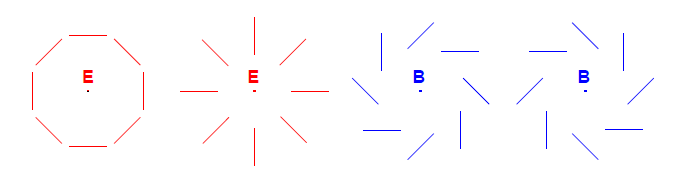
\includegraphics[width=\linewidth]{EBpicture.png}
  \caption{Typical E or B mode polarisation patterns. The electric and magnetic modes are distinguished by their behaviour under reflection}
\end{figure}

\subsubsection{Statistics}
Edited once



In this section we define the power spectra of interest. Since primordial perturbations from inflation are expected to be Gaussian, and since we expect linear theory to be a very good approximation in the early universe pre recombination, we also expect the small anisotropies in the CMB fields to be independent and Guassian, with zero mean. 

\begin{equation}
\langle T_{lm} \rangle = \langle E_{lm} \rangle = \langle B_{lm} \rangle = 0
\end{equation}

where we have redefined $T$ here to be the temperature anistropy instead of the absolute temperature. These three sets of moments define the full temperature and polarisation map. By gaussianity, all their statistical properties are contained in their power spectra, which by statistical isotropy take form:


\begin{equation}\begin{split}
\langle T_{lm}^*T_{l'm'} \rangle &= C^{TT}_l\delta_{ll'}\delta_{mm'}\\
\langle E_{lm}^*E_{l'm'} \rangle &= C^{EE}_l\delta_{ll'}\delta_{mm'}\\
\langle B_{lm}^*B_{l'm'} \rangle &= C^{BB}_l\delta_{ll'}\delta_{mm'}\\
\langle T_{lm}^*E_{l'm'} \rangle &= C^{TE}_l\delta_{ll'}\delta_{mm'}\\
\langle T_{lm}^*B_{l'm'} \rangle &= \langle E_{lm}^*B_{l'm'} \rangle = 0
\end{split}\end{equation}

The last line follows from the parity invariance of power spectra and the parity of T, E and B modes.

\begin{equation}
C_l^{XY} = \frac{1}{2l+1}\sum_m \langle X_{lm}^*Y_{l'm'}\rangle
\label{powerspectra}
\end{equation}

for $X,Y \in \{T, E,B\}$. For the case of $XY = EE, TT, BB$ these are in fact unbiased estimators also.



\subsection{The flat sky approximation}

The flat sky approximation is the small scale limit of the above discussion. It neglects the curvature of the sphere, allowing us to work instead with a standard flat space Fourier basis, instead of (spin-weighted) spherical harmonics. It is a reasonable approximation on small angular scales, and also provides a useful tool to give intuition about physical effects. It is also historically relevant: much of the early work on CMB polarisation focussed on this limit, before the techniques discussed above to deal with the full sky were discovered. 

Here, we'll describe how to get the small scale limit out of the full sky treatment.  We take $\unit{n}$ to be close to $\unit{z}$, and make the substitutions:

\begin{equation}
\begin{split}
Y_{lm}(\unit{n}) &\rightarrow e^{i\v{l}\cdot\unit{n}}\\
\sum_{lm} &\rightarrow \finttwo{l}
\end{split}
\end{equation}

leading to temperature anisotropies

\begin{equation}
T(\unit{n}) = \sum_{lm} T_{lm}Y_{lm}(\unit{n})\rightarrow \finttwo{l} T(\v{l})e^{i\v{l}\cdot\unit{n}}
\end{equation}

and spin weighted spherical harmonics becoming 

\begin{equation}\begin{split}
{}_2Y_{lm} &= \ltwo^\half\sr^2Y_{lm} \rightarrow \frac{1}{l^2}\sr^2e^{i\v{l}\cdot\unit{n}}\\
{}_{-2}Y_{lm} &= \ltwo^\half\sl^2Y_{lm} \rightarrow  \frac{1}{l^2}\sl^2e^{i\v{l}\cdot\unit{n}}
\end{split}\end{equation}

and so \ref{QUEB} for polarisation becomes

\begin{equation}\begin{split}
(Q+iU)(\unit{n}) &= -\finttwo{l} [E(\v{l})+iB(\v{l})]  \frac{1}{l^2}\sr^2e^{i\v{l}\cdot\unit{n}}\\
(Q+iU)(\unit{n}) &= -\finttwo{l} [E(\v{l})+iB(\v{l})] \frac{1}{l^2}\sl^2e^{i\v{l}\cdot\unit{n}}
\end{split}\end{equation}

In the small scale limit we can derive:

\begin{equation}\begin{split}
\frac{1}{l^2}\sr^2e^{i\v{l}\cdot\unit{n}} &= -e^{-2i(\phi-\phi_l)}e^{i\v{l}\cdot\unit{n}}\\
\frac{1}{l^2}\sl^2e^{i\v{l}\cdot\unit{n}} &= -e^{2i(\phi-\phi_l)}e^{i\v{l}\cdot\unit{n}}
\end{split}\end{equation}

where $\phi_\v{l}$ is the angle between So far we have been using the natural basis $\unit{e_\theta}, \unit{e_\phi}$ on the sphere. In the flat sky however we should instead consider a fixed basis $\unit{e_x}, \unit{e_y}$ orthonormal to $\unit{z}$. We may rotate between them using $Q'\pm iU' = e^{\mp 2i\phi}(Q\pm iU)$ derived earlier, and find that (dropping the prime label)

\begin{equation}\begin{split}
Q(\unit{n}) &= \finttwo{l} [E(l)\cos{2\phi_l}-B(l)\sin{2\phi_l}]  e^{i\v{l}\cdot\unit{n}}\\
U(\unit{n}) &= \finttwo{l} [E(l)\sin{2\phi_l}+B(l)\cos{2\phi_l}]  e^{i\v{l}\cdot\unit{n}}\\
\end{split}\end{equation}

or alternatively, E and B modes are related to Q and U modes by a rotation in fourier space, as how introduced in FTC lectures. 

\begin{equation}
\begin{pmatrix}
Q(\v{l})\\
U(\v{l}) 
\end{pmatrix}
=
\begin{pmatrix}
\cos{2\phi_\v{l}} & -\sin{2\phi_\v{l}}\\ 
\sin{2\phi_\v{l}} & \cos{2\phi_\v{l}}
\end{pmatrix}
\begin{pmatrix}
E(\v{l})\\
B(\v{l}) 
\end{pmatrix}
\end{equation}

or more compactly

\begin{equation}
(Q+iU)(\v{l}) = e^{2i\phi_\v{l}}(E+iB)(\v{l})
\end{equation}

\subsection{B Modes from Inflation}

Having discussed the relevant polarisation observables, we now wish to understand how inflation may generate them. The main goal of this section is to show that tensor perturbations source a non zero B mode polarisation, whose power spectrum depends on the primordial tensor power spectrum. \\

To completely understand the full photon distribution we must follow the evolution of the four stokes parameters, giving four distribution functions $f_s$, $s\in\{I,Q,U,V\}$. The original (unperturbed) distribution functions are $\bar{f}_I(\v{x},\v{p}, \tau)= [e^{\hbar \nu/k_b T(\tau)}-1]^{-1}$ and $\bar{f}_U=\bar{f}_Q=\bar{f}_V=0$, as the light is initially unpolarised. As mentioned previously, Thomson scattering does not induce any circular polarisation so $f_V$ remains 0 for all time and we need not consider it. Working to linear order in pertubation theory all fourier modes decouple, and we introduce first order pertubations as

\begin{equation}
\Delta_s(\v{k}, \v{p}, \tau) = 4f^{(1)}_s(\frac{\partial\bar{f}_I}{\partial \ln{T}})^{-1}
\end{equation}

We'll work in Fourier space throughout, focussing on a mode with wave vector $\v{k}$, which we may choose to be aligned with the $\unit{z}$ direction, and take the basis on which we evaluate $Q$ and $U$ to be the natural basis on the sphere: $(\unit{e_1}, \unit{e_2}) = (\unit{e_\theta}, \unit{e_\phi})$.\\

\subsubsection{Tensor (gravitational wave) pertubations}

We now turn to the gravitational wave background. As we saw earlier, there exist two independent polarizations $\xi_+$ and $\xi_\times$ of the gravitational wave for each $\v{k}$ mode. We choose to work instead with the following linear combinations

\begin{equation}
\xi^1 = (\xi^+ - i\xi^\times)/\sqrt{2} \qquad \xi^2 = (\xi^+ + i\xi^\times)/\sqrt{2}
\end{equation}

which, being linearly independent linear combinations of $\xi_s$ are also independent gaussian random variables, each having half of the total primordial tensor power spectra:

\begin{equation}
\langle \xi^{1*}(\v{k})\xi^{1}(\v{k'})\rangle=\langle \xi^{2*}(\v{k})\xi^{2}(\v{k'})\rangle=\half P_t(k)\delta(\v{k}-\v{k'})
\end{equation}
\begin{equation}
\langle \xi^{1*}(\v{k})\xi^{2}(\v{k'})\rangle=0
\end{equation}

Following the approach taken by Polnarev, we introduce related perturbations encapsulating the necessary angular dependence of the original perturbations, in terms of which  which the Boltzmann equations neatly decouple

\begin{equation}\begin{split}
\Delta_T(\tau,\unit{n},\v{k}) &= [(1-\mu^2) e^{2i\phi} \xi^1(\v{k})+(1-\mu^2) e^{-2i\phi} \xi^2(\v{k})]\tilde{\Delta_T}(\tau,\mu,k)\\
(\Delta_Q+i\Delta_U)(\tau,\unit{n},\v{k}) &=[(1-\mu)^2 e^{2i\phi} \xi^1(\v{k})+(1+\mu)^2 e^{-2i\phi} \xi^2(\v{k})]\tilde{\Delta_P}(\tau,\mu,k) \\
(\Delta_Q-i\Delta_U)(\tau,\unit{n},\v{k}) &=[(1+\mu)^2 e^{2i\phi} \xi^1(\v{k})+(1-\mu)^2 e^{-2i\phi} \xi^2(\v{k})]\tilde{\Delta_P}(\tau,\mu,k)
\end{split}\end{equation}

These satisfy

\begin{equation}\begin{split}
\tilde{\Delta}_T'+ik\mu \tilde{\Delta}_T &= -h' -\kappa'[\tilde{\Delta}_T - \Psi]\\
\tilde{\Delta}_P'+ik\mu\tilde{\Delta}_P &= -\kappa'[\tilde{\Delta}_P + \Psi]
\end{split}\end{equation}

where the source is

\begin{equation}
\Psi = \frac{1}{10}\tilde{\Delta}_{T0} + \frac{1}{7}\tilde{\Delta}_{T2} + \frac{3}{70}\tilde{\Delta}_{T4} - \frac{3}{5}\tilde{\Delta}_{P0} + \frac{6}{7}\tilde{\Delta}_{P2} - \frac{3}{70}\tilde{\Delta}_{P4}
\end{equation}


written in terms of multipole moments, defined for any function as $f(k, \mu) = \sum_l (2l+1)(-i)^lf_l(k)P_l(\mu)$ for $P_l(\mu)$ the order $l$ legendre polynomial. All derivatives are taken with respect to conformal time $\tau$. $h$ is the gravitational wave amplitude.\\

The \textit{optical depth} for Thomson scattering is given by the integral $\kappa(\tau) = \int_\tau^{\tau_0} an_e\sigma_T$ and denotes the probability for a photon not to scatter between conformal time $\tau$ and today $\tau_0$ as $e^{-\kappa}$. From this we see $\kappa'=-an_e\sigma_T$. Let us also introduce the \textit{visibility function} $g(\tau) = \kappa'e^{-\kappa}$, encoding the probability a photon last scattered at $\tau$. Integrating:

\begin{equation}
\int_0^{\tau_0} g d\tilde{\tau} = [-e^{-\kappa}]_0^{\tau_0} = 1
\end{equation}

using the limits $\kappa \rightarrow \infty$ as $\tau\rightarrow0$ (early times) and $\kappa \rightarrow 0$ as $\tau\rightarrow \infty$ (late times).\\




 The \textit{differential optical depth} for Thomson scattering is $-\kappa'=$, where $n_e$ is the electron density, and $\sigma_T$ is the Thomson cross section.  \\
something fishy with minus signs in optical depths here\\






We now use the `line of sight method' and formally integrate these first order linear ODEs, using an integrating factor. Introducing $x=k(\tau_0-\tau)$ we get  

\begin{equation}\begin{split}
\tilde{\Delta}_T(\tau_0,\mu,k) &= \int_0^{\tau_0} e^{ix\mu}S_T(k,\tau)\\
\tilde{\Delta}_P(\tau_0,\mu,k) &= \int_0^{\tau_0} e^{ix\mu}S_P(k,\tau)
\end{split}\end{equation}

where all the physics is hidden in the source terms:

\begin{equation}\begin{split}
S_T(k,\tau) &= -h'e^{-\kappa}+g\Psi\\
S_P(k,\tau) &= -g\Psi
\end{split}\end{equation}

where $g(\tau) = \kappa'e^{-\kappa}$ is the visibility function, peaking at the epoch of recombination. A simple approximation takes recombination to be instantaneous, at $\tau_*$, in which case $g(\tau) = \delta(\tau-\tau_*)$. Combining the last two results we attain expressions for the original T,Q,U pertubations we care about:



\begin{equation}\begin{split}
\Delta_T(\tau_0,\unit{n},\v{k}) &= [(1-\mu^2) e^{2i\phi} \xi^1(\v{k})+(1-\mu^2) e^{-2i\phi} \xi^2(\v{k})]\int_0^{\tau_0} e^{ix\mu}S_T(k,\tau)\\
(\Delta_Q+i\Delta_U)(\tau_0,\unit{n},\v{k}) &=[(1-\mu)^2 e^{2i\phi} \xi^1(\v{k})+(1+\mu)^2 e^{-2i\phi} \xi^2(\v{k})]\int_0^{\tau_0} e^{ix\mu}S_P(k,\tau)\\
(\Delta_Q-i\Delta_U)(\tau_0,\unit{n},\v{k}) &=[(1+\mu)^2 e^{2i\phi} \xi^1(\v{k})+(1-\mu)^2 e^{-2i\phi} \xi^2(\v{k})]\int_0^{\tau_0} e^{ix\mu}S_P(k,\tau)
\end{split}\end{equation}



The T result is what we want. For Q and U however are coordinate dependent quantities on the sphere, and so instead we work with $\tilde{E}$ and $\tilde{B}$. To do so, by \ref{EBmodes} all we need to do is act twice via our raising and lowering operators. We make use of \ref{+-2}, which conveniently pass through the source terms, which have no angular dependence. We get

\begin{equation}\begin{split}
\sl^2(\Delta_Q+i\Delta_U)(\tau_0,\unit{n},\v{k}) &= \xi^1(\v{k})e^{2i\phi}\int_0^{\tau_0}S_P(k,\tau)(\partial_\mu+\frac{2}{1-\mu^2})^2[(1-\mu^2)(1-\mu)^2 e^{ix\mu}]\\
&{} + \xi^2(\v{k})e^{-2i\phi}\int_0^{\tau_0}S_P(k,\tau)(\partial_\mu+\frac{2}{1-\mu^2})^2[(1-\mu^2)(1+\mu)^2 e^{ix\mu}]\\
&= \xi^1(\v{k})e^{2i\phi}\int_0^{\tau_0}S_P(k,\tau)(-\mathcal{E}(x)-i\mathcal{B}(x))[(1-\mu^2) e^{ix\mu}] \\
&{} + \xi^2(\v{k})e^{-2i\phi}\int_0^{\tau_0}S_P(k,\tau)(-\mathcal{E}(x)-i\mathcal{B}(x))[(1-\mu^2) e^{ix\mu}] not sure about this line
\end{split}\end{equation}

\begin{equation}\begin{split}
\sr^2(\Delta_Q-i\Delta_U)(\tau_0,\unit{n},\v{k}) &= \xi^1(\v{k})e^{2i\phi}\int_0^{\tau_0}S_P(k,\tau)(\partial_\mu-\frac{2}{1-\mu^2})^2[(1-\mu^2)(1+\mu)^2 e^{ix\mu}] \\ 
&{} + \xi^2(\v{k})e^{-2i\phi}\int_0^{\tau_0}S_P(k,\tau)(\partial_\mu-\frac{2}{1-\mu^2})^2[(1-\mu^2)(1-\mu)^2 e^{ix\mu}]\\
&= \xi^1(\v{k})e^{2i\phi}\int_0^{\tau_0}S_P(k,\tau)(-\mathcal{E}(x)+i\mathcal{B}(x))[(1-\mu^2) e^{ix\mu}] \\
&{} + \xi^2(\v{k})e^{-2i\phi}\int_0^{\tau_0}S_P(k,\tau)(-\mathcal{E}(x)+i\mathcal{B}(x))[(1-\mu^2) e^{ix\mu}] not sure about this line
\end{split}\end{equation}

where we have introduced differential operators, which will save us some work very soon.

\begin{equation}
\mathcal{E}(x)=-12+x^2(1-\partial^2_x)-8x\partial_x \qquad \mathcal{B}(x) = 8x+2x^2\partial_x
\end{equation}

Plugging these into \ref{EBmodes} we find our final results for each fourier mode to be:

\begin{equation}\begin{split}
\Delta_T(\tau_0,\unit{n},\v{k}) &= [(1-\mu^2) e^{2i\phi} \xi^1(\v{k})+(1-\mu^2) e^{-2i\phi} \xi^2(\v{k})]\int_0^{\tau_0} e^{ix\mu}S_T(k,\tau)\\
\Delta_{\tilde{E}}(\tau_0,\unit{n},\v{k}) &= [(1-\mu^2) e^{2i\phi} \xi^1(\v{k})+(1-\mu^2) e^{-2i\phi} \xi^2(\v{k})]\mathcal{E}(x)\int_0^{\tau_0} e^{ix\mu}S_P(k,\tau)\\
\Delta_{\tilde{B}}(\tau_0,\unit{n},\v{k}) &= [(1-\mu^2) e^{2i\phi} \xi^1(\v{k})+(1-\mu^2) e^{-2i\phi} \xi^2(\v{k})]\mathcal{B}(x)\int_0^{\tau_0} e^{ix\mu}S_P(k,\tau)
\label{LoSfourier}
\end{split}\end{equation}

The complete solution requires integration over all fourier modes, which evolve independently. Note the fourier factor is omitted since we measure each mode from the same spatial position $\v{x}$.

\begin{equation}\begin{split}
\Delta_T(\tau_0,\unit{n}) &= \fint{k} \Delta_T(\tau_0,\unit{n},\v{k})\\
\Delta_{\tilde{E}}(\tau_0,\unit{n}) &= \fint{k}\Delta_{\tilde{E}}(\tau_0,\unit{n},\v{k})\\
\Delta_{\tilde{B}}(\tau_0,\unit{n}) &= \fint{k}\Delta_{\tilde{B}}(\tau_0,\unit{n},\v{k})
\end{split}\end{equation}

If we had chosen to work with Q and U here, in order to sum up Fourier modes with respect to a fixed basis with respect to the sphere, we would need to rotate each $Q\pm iU$ $\v{k}$ mode by a $\v{k}$ and $\unit{n}$ dependent phase (since we aligned $\v{k}$ with $\unit{z}$). This was a complication in early attempts to characterise the CMB polarisation beyond the flat sky regime, and we have avoided it through our definition of rotationally invariant E and B modes.\\

We see tensor perturbations have induced both E and B modes.

\subsubsection{Tensor power spectra}

Since the form of these are so similar, we can compute the TT, EE and BB correlation functions all in one go. We can also, with more work, verify that T does not correlate with E or B.\\

We'll begin by calculating the TT power spectrum $C_l^{TT}$ sourced by tensor pertubations. Recalling the definition of the angular power spectrum, we first require the spherical multipole coefficients $T_{lm}$  

\begin{equation}
T_{lm} = \int d\Omega Y_{lm}^*(\unit{n})\Delta_T(\tau_0,\unit{n})
\end{equation}

From \ref{powerspectra} we can write 

\begin{equation}\begin{split}
C_l^{TT} &= \frac{1}{2l+1}\sum_m \langle T_{lm}^*T_{lm} \rangle \\
&= \frac{1}{2l+1} \sum_m [\int d\Omega Y_{lm}^*(\unit{n})\int d^3k\int_0^{\tau_0}d\tau S_T(\tau,k)e^{ix\mu}]^*
[\int d\Omega Y_{lm}^*(\tilde{\unit{n}})\int d^3\tilde{k}\int_0^{\tau_0}d\tilde{\tau}S_T(\tau,\tilde{k})e^{i\tilde{x}\tilde{\mu}}]\\
&\times
\langle [(1-\mu^2) e^{2i\phi} \xi^1(\v{k})+(1-\mu^2) e^{-2i\phi} \xi^2(\v{k})]^*[(1-\tilde{\mu}^2) e^{2i\tilde{\phi}} \xi^1(\v{\tilde{k}})+(1-\tilde{\mu}^2) e^{-2i\tilde{\phi}} \xi^2(\v{\tilde{k}})] \rangle
\end{split}\end{equation}

The expectation value evaluates to

\begin{equation}\begin{split}
&(1-\mu^2)(1-\tilde{\mu}^2)[\langle\xi^{1*}(\v{k})\xi^1(\v{\tilde{k}})\rangle e^{2i\tilde{\phi}-2i\phi}+\langle\xi^{2*}(\v{k})\xi^2(\v{\tilde{k}})\rangle e^{-2i\tilde{\phi}+2i\phi}]\\
&~ (1-\mu^2)(1-\tilde{\mu}^2)P_t(k)\delta(\v{k}-\v{\tilde{k}})\half(e^{2i\tilde{\phi}-2i\phi}+e^{2i\phi-2i\tilde{\phi}}
\end{split}\end{equation}

and so the final expression can be written conveniently as 

\begin{equation}\begin{split}
C_l^{TT} = \frac{1}{2l+1} \int k^2 dk P_t(k) \sum_m \bigg| \int d\Omega Y^*_{lm}(\unit{n}) \int_0^{\tau_0} S_T(k,\tau)(1-\mu^2)e^{2i\phi}e^{ix\mu} \bigg|^2
\end{split}\end{equation}

To evaluate this, we use the expression $Y_{lm} = [\frac{(2l+1)(l-m)!}{4\pi(l+m)!}]^\half P_l^m(\mu)e^{-im\phi}$ for spherical harmonics in terms of legendre polynomials, and note that the $\phi$ integral vanishes unless $m=2$, in which case it gives $2\pi$. So we get 

\begin{equation}\begin{split}
C_l^{TT} = 4\pi^2\ltwof \int k^2 dk P_t(k) \bigg|  \int_0^{\tau_0} S_T(k,\tau)\int_{-1}^1 d\mu P_l^2(\mu)(1-\mu^2)e^{ix\mu} \bigg|^2
\end{split}\end{equation}

To evaluate the $\mu$ integral, we use $P^m_l(\mu)=(-1)^m(1-\mu^2)^{m/2}(\partial_\mu)^mP_l(\mu)$ and so


\begin{equation}\begin{split}
\int d\mu P_l^2(\mu)(1-\mu^2)e^{ix\mu} 
&= \int d\mu(1-\mu^2)^2 \partial_\mu^2P_l(\mu)e^{ix\mu}\\
&= \int d\mu \partial_\mu^2P_l(\mu)(1+\partial_x^2)^2e^{ix\mu}\\
&= \int d\mu P_l(\mu)(1+\partial_x^2)^2(x^2e^{ix\mu})\\
&= 2i^l(1+\partial_x^2)^2(x^2j_l(x))\\
&= 2i^l(\frac{j_l(x)}{x^2})
\end{split}\end{equation}

making use of $\int d\Omega Y_{lm}^*(\unit{n})e^{ix\mu} = \sqrt{4\pi(2l+1)}i^l j_l(x) \delta_{m0}$ and $Y_{l0} = \sqrt{\frac{2l+1}{4\pi}}P_l(\mu)$. In the final line we used the ODE for spherical bessel functions: $j_l''+\frac{2j_l'}{x}+(1-\frac{l(l+1)}{x^2}j_l)=0$.\\

Thus our final result is:

\begin{equation}\begin{split}
C_l^{TT} = (4\pi)^2\ltwof \int k^2 dk P_t(k) \bigg|  \int_0^{\tau_0} S_T(k,\tau)\frac{j_l(x)}{x^2} \bigg|^2
\end{split}\end{equation}

Now we abuse the similarity of expressions in \ref{LoSfourier} to write down the EE and BB power spectra. The angular dependence of $\Delta_{\tilde{E}}$ and $\Delta_{\tilde{B}}$ are exactly the same as those of $\Delta_T$. The expressions differ only in the $\mathcal{E}$ and $\mathcal{B}$ operators, acting seperately on each $\v{k}$ mode, which can be applied after the angular integrals are performed. We lose the $l$ dependent factor in front by converting from $\tilde{E}, \tilde{B}$ to $E,B$, using \ref{EBtwiddle}


\begin{equation}\begin{split}
C_l^{EE} &= (4\pi)^2 \int k^2 dk P_t(k) \bigg|  \int_0^{\tau_0} S_T(k,\tau)\mathcal{E}(x)\frac{j_l(x)}{x^2} \bigg|^2\\
&= (4\pi)^2\int k^2 dk P_t(k) \bigg|  \int_0^{\tau_0} S_T(k,\tau)[-j_l(x) +j_l''(x)+\frac{2j_l(x)}{x^2} + \frac{4j_l'(x)}{x}]\bigg|^2\\
C_l^{BB} &= (4\pi)^2 \int k^2 dk P_t(k) \bigg|  \int_0^{\tau_0} S_T(k,\tau)\mathcal{B}(x)\frac{j_l(x)}{x^2} \bigg|^2\\
&= (4\pi)^2\int k^2 dk P_t(k) \bigg|  \int_0^{\tau_0} S_T(k,\tau)[2j_l'(x)+\frac{4j_l(x)}{x}]\bigg|^2
\label{primordialBmodes}
\end{split}\end{equation}


\subsubsection{Scalar (density) pertubations}

One can go through an almost identical, and actually simpler, process to derive analgous power spectra sourced by scalar pertubations. We omit these here, but will explain the reason why they produce no B mode polarisation. As before, we work in fourier space with wave vector $\v{k}$, which we may choose to be aligned with the $\unit{z}$ direction, and take the basis on which we evaluate $Q$ and $U$ to be the natural basis on the sphere: $(\unit{e_1}, \unit{e_2}) = (\unit{e_\theta}, \unit{e_\phi})$. The angular dependence of the Boltzmann equations are only in $\mu=\v{k}\cdot\unit{n}$, and thus we have azimuthal symmetry, or $\phi$ independence, causing only the Q stokes parameter to be generated. Another way to say the same thing is that the polarisation eigenvector must be proportional to $\unit{e_\theta}$, which by the form of polarisation matrix forces $U=0$. Now by \ref{EBmodes}, we see if $U=0$, then $B(\unit{n})$ is identically 0. Physically speaking, the reason tensor perturbations induce both Q and U polarisation, is because of the additional degree of freedom we have in tensor modes compared to scalar modes.


\subsection{Summary}

We have seen that primordial pertubations induce characteristic signals in the CMB. We find

\begin{itemize}
\item Scalar pertubations create only E modes, and no B modes
\item Tensor pertubations create both E and B modes
\end{itemize}


We explicitly showed the second, and gave a heuristic argument for the first. The only significant source of primordial B modes is through tensor pertubations. The line-of-sight method is computationally efficient, as having numerically integrated the boltzmann heirachy derived by expanding \ref{} in terms of multipole moments, once can compute the power spectra easily.


Additionally

\begin{itemize}
\item Vector pertubations create mostly B modes, but their contribution is expected to be small
\end{itemize}



Plot from somewhere???



 We explicitly calculated the power spectra induced by tensor modes in the computationally efficient "line of sight" method. 


metric tensor pertubations produce a B mode signal in the CMB polarisation, unlike scalar pertubations. Four angular power spectra depend on tensor pertubations, though three of these observables also depend also on scalar perturbations, since E and T are also sourced by  these. As we discussed in the inflation chapter, we know this is at least an order of magnitude larger a signal, likely more. Therefore B mode polarisation provides the most promising route to detecting primordial tensor pertubations. Note we have only so far discussed the early universe. As we will see in the next chapter, late time effects also generate a B mode signal, which for the purposes of studying inflation is a large is an obstacle, though some of these extra B modes provide interesting insights, useful elsewhere.

Assuming we have a clean measurement of the CMB polarisation, with foregrounds suffiecently well removed, we can infer properties of inflation only if we are sure the only B modes present are due to primordial tensor pertubations. We give some examples of such effects here:

[CMBpol] Topological defects and cosmic strings: Certain classes of GUTs for inflation involve phase transitions near the end of inflation that produce topological defects. 

topological defects -> vector pertubations



Gravitational lensing: The effects above are speculative, their effects are in general very model dependent. On the other hand lensing is something we know to occur, and its effects are easily quantified.So far we have assumed photons last scattered at recombination have travelled to us unimpeded. This can be seen directly through the dependence of derived temperature, E and B mode  power spectra dependence on the visibility function, which has support only in the epoch of recombination. CMB photons experience late time deflections, as a result of the intervening large scale structure present between redshift 0 and recombination ($z ~ 1100$). We discuss this in some detail in the next chapter.




\section{Observational Challenges}

We have seen an inflationary B mode signal provides strong evidence for inflation, and so much work is being put into trying to detect them. This proves to be rather a difficult endeavour. While temperature anistropies are week, polarisation fluctuates are weaker. Additionally, there are two main issues to overcome, both due to sources of B modes outside of the primary CMB.


\subsection{Foregrounds}

The CMB offers fascinating insights into the early universe. Here we turn our attention towards how to actually study the CMB. It's a little bit like trying to find a needle in a haystack. Firstly, instrumental noise and imperfections could comprimise the sort of tiny signals we will be required to detect to find B modes. Even in the absence of these purely experimental issues, there exist many astrophysical or atmospheric foregrounds that contaminate our CMB signal. In this section we give an overview of the relevant foregrounds for the study of polarisation, and describe how we may go about dealing with them.\\

Recall first that the CMB is a near perfect black body emitter, with a characteristic frequency profile given by the Planck distribution

\begin{figure}[h]
  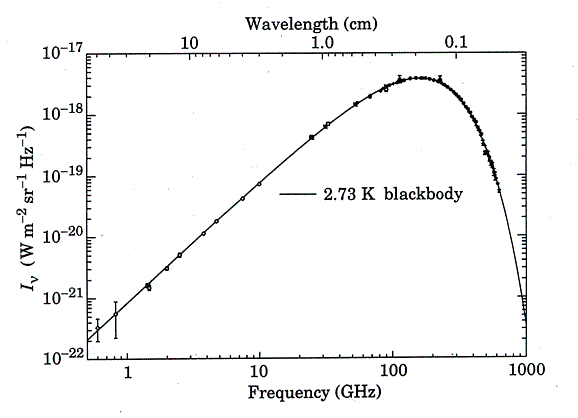
\includegraphics[width=0.7\linewidth]{cmbspectrum1.png}
  \centering
  \caption{https://webhome.phy.duke.edu/~kolena/cmb.html the CMB spectrum as measured by the COBE sattelite, matches that of a black body emitter at the CMB temperature}
\end{figure}

peaking at about 160Ghz. Foregrounds can broadly be seperated into atmospheric, galactic, or extragalactic. Each type have their own frequency dependence, and degree of polarisation. Those contributing at CMB frequencies are summarised in \ref{foregrounds}. We see the main contaminants for our studies of polarisation are galactic in origin, from synchrotron emission at low frequencies below 100Ghz, and thermal dust at higher frequencies. The other contaminants listed in the top panel, such as spinning dust, foruturn out to not be significantly polarised so don't pose too much of an issue. Additionally, for ground based experiments, there are several atmospheric effects.


\begin{figure}[h]
  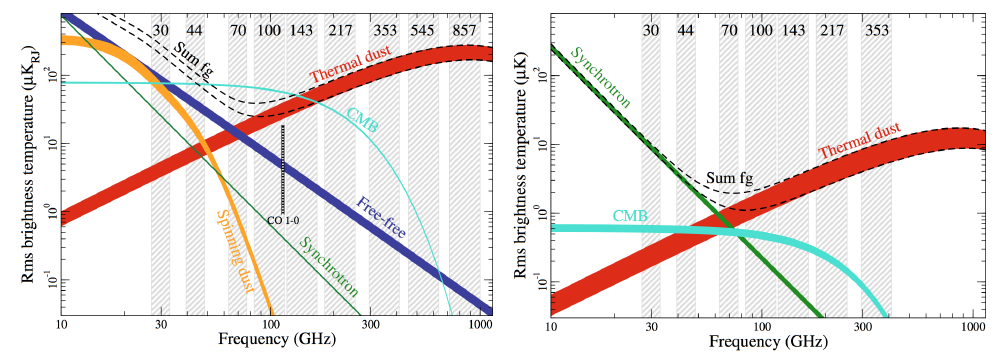
\includegraphics[width=0.5\linewidth]{foregrounds.png}
  \caption{Spectral energy distributions (SED) of relevant astrophysical foregrounds. The top panel are the main contributions to temperature, and the bottom, for polarisation. The shaded bars indicate the observation frequencies for the Planck satellite, and the upper and lower limits correspond to masks with different sky fractions used (81 and 93\%). Taken from Planck (2016b fig 51) }
  \label{foregrounds}
\end{figure}

This really is a large problem! The expected B mode signal, even for a relatively large value of $r\approx0.1$ falls below the average polarised foreground level on the full sky at all CMB frequencies.  \\

\textbf{Atomospheric effects}: Absorption lines from oxygen at 60 and 120 Ghz, and water vapour at 20 and 18Ghz limit access to the microwave sky. Thermal emission from the atmosphere is unpolarised, though Zeeman splitting of oxygen lines in Earth's magnetic field leads to polarized emission, which is primarily circularly polarized. While the CMB is not expected to be circularly polarized, instrumental issues could lead to a $\approx 0.01\%$ circular-to-linear polarisation conversion, which could lead to a measured B mODE signal orders of magnitude larger than if $r=0.01$, say. Backscattering of thermal radiation emitted by the earths surface off ice  crystal clouds in the troposphere may also give B mode signals larger than the expected CMB B mode signal. Some of these effects will be harder to remove than others: for example the signal from ice clouds would be inhomogeneous and hard to predict.\\

\textbf{Galactic Synchrotron emission}: This emission is produced by acceleration of charged particles in interstellar magnetic fields. Via multi frequency measurements via the CMB satellites (WMAP and Planck), one find a very good fit to SED $T_d(\nu) \propto \nu^{\beta_s}$ with $\beta_s \approx -3$, and varying slightly over the sky, since it depends on the particular acceleration of charged particles. Theoretically, a high degree of polarisation is expected.\\

\textbf{Galactic Dust}: This emission is produced due to presence of dust grains in the interstellar medium (ISM). In dense regions of star formation, UV radiation from newly formed stars heats up nearby dust, which radiate strongly polarised light in the IR and microwave frequencies. The grain size and dust temperature determine the spectral properties of the radiation, which can be fitted well to a modified black body emission spectrum

\begin{equation}
T_d(\nu) \propto \nu ^ {\beta_d+1}[e^{\nu/T}-1]^{-1}
\end{equation}

Measurements from Planck show $T_d$ and spectral parameter $\beta_d$ vary over the sky, with average values differing slightly in and out of the galactic plane. While no region of the sky was found to be sufficiently clean of dust to require no foreground removal for clean B mode measurements, Planck did identify certain patches of the sky with considerably lower foreground amplitudes, which may be of use in future CMB missions. \\


The statistical algorithms and methods designed to separate these foregrounds from the clean CMB (the primary signal plus secondary effects) are known as CMB component separation (Delabrouille and Cardoso, 2009), make use of several datasets. They can be grouped into two classes. Non blind methods attempt to make use of the known spectral frequency properties of certain foregrounds, to disentangle them from the background CMB. Blind methods on the other hand assume little or no prior information about the form of the foregrounds, instead relying on their statistics: different foregrounds should be statistically independent, and the clean CMB should be statistically simple - it is gaussian.\\

Proper foreground removal is very important. In order to detect a primordial B mode signal at $r=0.01$ at a $3\sigma$ significance for example, we must only have a $1\%$ level of residual foregrounds. It is easy to go wrong. In March 2014 the BICEP2 Collaboration reported detection of B-mode power at 150 GHz and in the range $40<l<100$, in excess of that expected from the other observational issue of lensing (see next section). The B-mode signal was found have an amplitude greater than that expected from foregrounds, and not to correlate with them either. This would have been huge, however unforutnately, under further scrutiny arguments were made that extraordinary implications of this measurement attracted considerable scrutiny, and arguments were made that uncertainties in the various dust templates may have been underestimated. By cross correlating further BICEP2/Keck and Planck data, it was discovered that the entire excess B mode could be attributed to dust. 



\subsection{CMB Lensing}

Gravitational lensing is a second order effect, intuitively because it is a combination of two first order effects: it deflects the photon path away from its straight line geodesic, as a result of clustering of matter between last scattering and today. Being second order, we dropped the term in the boltzmann equation describing when we linearised. In the linear regime each fourier mode evolves independently, but lensing mixes these fourier modes, making the statistics of the lensed sky more complicated than those of the unlensed one. \\

We treat lensing in the `weak lensing' regime, where images (and other fields on the sphere) experience a small shift compared to the original unlensed field. The effect of gravitational lensing is greatest when the lens is massive, and close to the source. While lenses for the purposes of CMB some lenses certainly are massive, they are relatively far from the $z~1100$ source, since structure doesn't form in the universe until a much later time. The contrary `strong lensing' regime is also very interesting, though not relevant here.\\

Lensing effects all three of our observable CMB fields: the temperature fluctuation $\Theta$, and Stokes parameters $Q$ and $U$, and in doing so also the derived physical $E$ and $B$ fields in a way that will be made precise later. It has the effect of locally (i.e. on small patches of the sky) sqaushing and stretching the CMB, shifting local power spectra left or right. Summing over many patches we see a small smoothing of acoustic oscillations in the temperature and E mode spectra at several percent. \\

Importantly, it also has the effect of converting some primordial E modes to lensed B modes, which we demonstrate and quantify in the flat sky limit. This obscures the primordial B mode signal, and so is a nuisance in terms of early universe physics. However, lensing provides a probe of the matter distribution universe out to much larger redshifts than currently possible through galaxy surveys. One can extract a lot of information from this ...........

\subsubsection{Mathematical Description of Lensing}

The mathematical formalism to used to describe lensing is rather simple. From general relativity and a flat\footnote{similar expressions exist in positive and negative curvature universes} FLRW metric, one can derive an expression for the displacement vector or angle $\v{\alpha}$ on the sphere, dependent on observed direction $\unit{n}$, by which the lensed and unlensed fields differ:

\begin{equation}
\tilde{X}(\unit{n}) = X(\unit{n}+\v{\alpha})
\end{equation}

\begin{equation}
\v{\alpha} = -2 \int_0^{\chi_*}d\chi \frac{\chi_*-\chi}{\chi_*\chi}\nabla_{\unit{n}}\Psi(\chi\unit{n},\tau_0-\chi)
\end{equation}

where $X$ is an observable field: $X \in \{ \Theta, U, V\}$, $\chi$ is conformal distance, $\tau_0-\chi$ is the conformal time at which the photon was at position $\chi\unit{n}$, $\nabla_{\unit{n}}$ is the angular derivative, or covariant derivative on the sphere, and $\Psi$ is the Weyl potential, defined in terms of \ref{perturbmetric} as $\Psi =\half (\psi+\phi)$. This quantity is related to matter perturbations by what is commonly known as the Poisson Equation, derived from Einstein's equations:

\begin{equation}
\nabla^2\Psi = 4\pi G\bar{\delta\rho}
\end{equation}

where $\bar{\delta\rho}$ is the comoving total density perturbation, evaluated in its rest frame, and we have assumed no anisotropic stress. It is convenient to write the deflection angle instead in terms of a lensing potential:

\begin{equation}\begin{split}
\psi(\unit{n}) &= -2 \int_0^{\chi_*}d\chi \frac{\chi_*-\chi}{\chi_*\chi}\Psi(\chi\unit{n},\tau_0-\chi)\\
\v{\alpha} &= \nabla \psi
\end{split}\end{equation}

One may worry about the lensing potential being divergent as $\chi \rightarrow 0$. We can amend this by setting the monopole of $\psi$ to 0, without modifying $\v{\alpha}$. 

\subsubsection{Lensing Potential power spectrum}

In the calculation of lensed power spectra, we will need the lensing potential power spectrum. Here we derive an expression for it, showing as expected it is simply a weighted matter power spectrum. We'll make use of fourier space the expression

\begin{equation}
\langle \Psi(\v{k},\tau,\tau')\Psi^*(\v{k}',\tau,\tau')\rangle=\frac{2\pi}{k^3}\Delta^2_\Psi(k,\tau,\tau')(2\pi)^3\delta(\v{k}-\v{k}')
\end{equation}

and so 

\begin{equation}\begin{split}
\langle \psi(\unit{n})\psi(\unit{'n}) \rangle &= 4\int d\chi \int d\chi'(\frac{\chi_*-\chi}{\chi_*\chi})(\frac{\chi_*-\chi'}{\chi_*\chi'}\fint{k}\frac{2\pi^2}{k^3}\delta^2_\Psi(k,\tau,\tau')e^{i\v{k}\cdot\v{x}}e^{-i\v{k}\cdot\v{x'}}\\
&= 16\pi \sum_{ll'mm'}\int d\chi \int d\chi'(\frac{\chi_*-\chi}{\chi_*\chi})(\frac{\chi_*-\chi'}{\chi_*\chi'}\int \frac{dk}{k}j_l(k\chi)j_{l'}(k\chi')Y_{lm}(\unit{n})Y^*_{l'm'}(\unit{n}')\delta_{ll'}\delta{mm'}
\end{split}\end{equation}

where we have made use of the Rayleigh Plane Wave identity with $\v{x}=\chi\unit{n}$

\begin{equation}
e^{i\v{k}\cdot\v{x}} = 4\pi\sum_{lm}i^lj_l(k\chi)Y_{lm}^*(\unit{n})Y_{lm}(\unit{k})
\end{equation}

and done the angular $\unit{k}$ using orthogonality of spherical harmonics. Finally we expand

\begin{equation}
\psi(\unit{n}) = \sum_{lm}\psi_{lm}Y_{lm}(\unit{n})
\end{equation}

and recalling the definition of $C_l^\psi$:

\begin{equation}
\langle \psi_{lm}\psi_{l'm'}^* \rangle = \delta_{ll'}\delta_{mm'}C_l^\psi
\end{equation}

we can read off the power spectrum:

\begin{equation}
C_l^\psi = 16\pi int_0^{\chi_*} d\chi \int_0^{\chi_*} d\chi' \int \frac{dk}{k} (\frac{\chi_*-\chi}{\chi_*\chi})(\frac{\chi_*-\chi'}{\chi_*\chi'}\Delta^2_\Psi(k, \tau_0-\chi, \tau_0-\chi')
\end{equation}

Finally we may relate the scale invariant power spectrum of $\Psi$ to that of $\bar{\delta}$ via the fourier transforming the Poisson Equation:

TO DO

\subsubsection{Lensing of B modes} 

We calculate in this section, in the flat sky regime, the effect lensing has on temperature, E mode, and importantly, B mode power spectra. 

We'll perform the calculation explicitly for temperature, with the polarisation calculations following similarly. We use here the series expansion approach, which gives good intuition and qualitatively correct results, though is not a good approximation on all scales. For larger scales a real space correlation function approach is used. In the series expansion approach we may expand

\begin{equation}
\tilde{\Theta(\unit{n}}) = \Theta(\unit{n}+\nabla\psi) =\Theta(\unit{n})+\nabla^a\psi(\unit{n})\nabla_a\Theta(\unit{n})+\half\nabla^a\psi(\unit{n})\nabla^b\psi(\unit{n})\nabla_a\nabla_b\Theta(\unit{n})
\end{equation}

Fourier transforming the above equation and using the convolution theorem we obtain

\begin{equation}\begin{split}
\tilde{\Theta}(\v{l}) &= \Theta(\v{l}) - \finttwo{l_1} \v{l_1}\cdot(\v{l}-\v{l_1})\Theta(\v{l_1})\psi(\v{l}-\v{l_1}) -\half \finttwo{l_1}\finttwo{l_2}\v{l_1}\cdot(\v{l_1}+\v{l_2}-\v{l})\v{l_1}\cdot\v{l_2}\Theta(\v{l_1})\psi(\v{l_2})\psi^*(\v{l_1}+\v{l_2}-\v{l})\\
&= \Theta(\v{l}) - \finttwo{l_1} \Theta(\v{l_1})L(\v{l},\v{l_1})
\label{lensedtemp}
\end{split}\end{equation}

making use of $\psi(\v{l})=\psi^*(-\v{l})$, and where we have defined the lensing kernel

\begin{equation}
L(\v{l},\v{l_1}) = \v{l_1}\cdot(\v{l}-\v{l_1})\psi(\v{l}-\v{l_1})+\finttwo{l_2}\v{l_1}\cdot(\v{l_1}+\v{l_2}-\v{l})\v{l_1}\cdot\v{l_2}\psi(\v{l_2})\psi^*(\v{l_1}+\v{l_2}-\v{l})\\
\end{equation}

Now we may calculate the (lensed) power spectrum of temperature perturbations to lowest order in the lensing potential power spectrum, defined as:

\begin{equation}
\langle \Theta^*(\v{l})\Theta(\v{l}')\rangle = (2\pi)^2\delta(\v{l}-\v{l}')C_l^{\Theta\Theta}
\end{equation}

using the fact that $\Theta$ and $\psi$ don't correlate, and Wick's theorem

\begin{equation}\begin{split}
\tilde{C}_l^{\Theta \Theta} &\approx C_l^{\Theta \Theta}+\finttwo{l_1}[ \v{l_1}\cdot(\v{l}-\v{l_1}]^2 C^\psi_{|\v{l}-\v{l_1}|}C_{l_1}^{\Theta\Theta} - C_l^{\Theta\Theta}\finttwo{l_1} [\v{l}\cdot\v{l_1}]^2C_{l_1}^{\psi\psi}\\
&=(1-l^2R^\psi)C_l^{\Theta\Theta}+\finttwo{l_1}[ \v{l_1}\cdot(\v{l}-\v{l_1}]^2 C^{\psi}_{|\v{l}-\v{l_1}|}C_{l_1}^{\Theta\Theta}
\end{split}\end{equation}

where we have defined

\begin{equation}
R^\psi = \frac{1}{4\pi}\int \frac{dl}{l} l^4 C_l^{\psi\psi}
\end{equation}

this gives our final lensed spectrum. SOME ANALYSIS OF LIMITING BEHAVIOUR

For polarisation, the calculation is rather similar. Recall that in the flat sky limit we must rotate Q and U fourier modes into E and B modes as:

\begin{equation}\begin{split}
(Q\pm iU(\unit{n}) := P_{\pm} (\unit{n}) &= \finttwo{l}(E(\v{l})\pm i B(\v{l}))e^{\pm 2i\phi_{\v{l}}}e^{i\v{l}\cdot\unit{n}}\\
\Leftrightarrow  P_{\pm}(\v{l}) &= (E(\v{l})\pm i B(\v{l}))e^{\pm 2i\phi_{\v{l}}}
\label{relationship}
\end{split}\end{equation}

Now lensing acts on $P_{\pm}$ exactly as it did on the temperature field 

\begin{equation}
\tilde{P_{\pm}(\unit{n}}) = P_{\pm}(\unit{n}+\nabla\psi) =P_{\pm}(\unit{n})+\nabla^a\psi(\unit{n})\nabla_aP_{\pm}(\unit{n})+\half\nabla^a\psi(\unit{n})\nabla^b\psi(\unit{n})\nabla_a\nabla_bP_{\pm}(\unit{n})
\end{equation}

which in fourier space gives

\begin{equation}
\tilde{P}_{\pm}(\v{l}) = P_{\pm} - \finttwo{l_1} P_{\pm}(\v{l_1})L(\v{l},\v{l_1})
\end{equation}

Finally to we use the relationship \ref{relationship} between $P_\pm$ and $E$ and $B$ modes twice:

\begin{equation}\begin{split}
\tilde{E}(\v{l})\pm i\tilde{B}(\v{l}) &= e^{-2i\phi_\v{l}}\tilde{P}_{\pm}(\v{l})\\
&=e^{\mp 2i\phi_\v{l}}(P_{\pm}(\v{l}) - \finttwo{l_1} P_{\pm}(\v{l_1})L(\v{l},\v{l_1}))\\
&=E(\v{l})\pm iB(\v{l})-\finttwo{l_1} e^{\pm 2i(\phi_\v{l_1}-\phi_\v{l})}(E(\v{l_1})\pm iB(\v{l_1}))L(\v{l},\v{l_1})
\label{lensedEBmodes}
\end{split}\end{equation}

%&=e^{\mp 2i\phi_\v{l}}(e^{\pm 2i\phi_\v{l}}(E(\v{l})\pm iB(\v{l}))-\finttwo{l_1} e^{+2i\phi_\v{l_1}}(E(\v{l_1})\pm iB(\v{l_1}))L(\v{l},\v{l_1}))\\


From this, we may calculate (lensed) power spectra for E and B (and the = TE cross correlation), defined on the flat sky as :

\begin{equation}
\langle E^*(\v{l})E(\v{l}')\rangle = (2\pi)^2\delta(\v{l}-\v{l}')C_l^{EE} \qquad \langle B^*(\v{l})B(\v{l}')\rangle = (2\pi)^2\delta(\v{l}-\v{l}')C_l^{BB}
\end{equation}


Schematically, this calculation is similar to that for lensed temperature perturbations, and we pick up identical terms. By correlating $\tilde{E}(\v{l})\pm i\tilde{B}(\v{l})$ with itself and $\tilde{E}(\v{l})\mp i\tilde{B}(\v{l})$ we obtain

\begin{equation}\begin{split}
\tilde{C}_l^{EE}+\tilde{C}_l^{BB} &\approx C_l^{EE}+C_l^{BB}+\finttwo{l_1}[ \v{l_1}\cdot(\v{l}-\v{l_1})]^2 C^\psi_{|\v{l}-\v{l_1}|}(C_{l_1}^{EE}+C_{l_1}^{BB}) - (C_{l}^{EE}+C_{l}^{BB})\finttwo{l_1} [\v{l}\cdot\v{l_1}]^2C_{l_1}^{\psi\psi}\\
\tilde{C}_l^{EE}-\tilde{C}_l^{BB} &\approx C_l^{EE}-C_l^{BB}+\finttwo{l_1}e^{4i(\phi_{\v{l_1}}-\phi_\v{l})}[ \v{l_1}\cdot(\v{l}-\v{l_1})]^2 C^\psi_{|\v{l}-\v{l_1}|}(C_{l_1}^{EE}-C_{l_1}^{BB}) - (C_{l}^{EE}-C_{l}^{BB}\finttwo{l_1} )[\v{l}\cdot\v{l_1}]^2C_{l_1}^{\psi\psi}
\end{split}\end{equation}

A similar calculation gives the $\tilde{C}_l^{EB}$. The integrals are actually all real (WHY?), and so we may replace the exponentials by cosines. Altogether we get:

\begin{equation}\begin{split}
\tilde{C}_l^{EE} &= (1-l^2R^\psi)C_l^{EE}+\half \finttwo{l_1}[ \v{l_1}\cdot(\v{l}-\v{l_1})]^2 C^\psi_{|\v{l}-\v{l_1}|}\\
& \times [(C_{l_1}^{EE}+C_{l_1}^{BB})+\cos{4(\phi_\v{l_1}-\phi_\v{l})}(C_{l_1}^{EE}+C_{l_1}^{BB})]\\
\tilde{C}_l^{BB} &= (1-l^2R^\psi)C_l^{BB}+\half \finttwo{l_1}[ \v{l_1}\cdot(\v{l}-\v{l_1})]^2 C^\psi_{|\v{l}-\v{l_1}|}\\
& \times [(C_{l_1}^{EE}+C_{l_1l}^{BB})-\cos{4(\phi_\v{l_1}-\phi_\v{l})}(C_{l_1}^{EE}+C_{l_1}^{BB})]\\
\label{lensedBmodes}
\end{split}\end{equation}

Here comes the key point: even if $C_{l}^{BB}$ is zero, i.e. we have no B modes sourced by primordial inflationary gravitational waves - lensing creates some. This has important consequences for the detectability of B modes.\\

Tensor modes would generate their largest signal on large scales or small $\v{l}$, so we seek to understand lensing B modes in that regime. Taking $C_l^{BB}=0$ we find for $|\v{l}| << |\v{l_1}|$ that 

\begin{equation}\begin{split}
\tilde{C}_l^{BB} &= \half \finttwo{l_1}[ \v{l_1}\cdot(\v{l}-\v{l_1})]^2 C^\psi_{|\v{l}-\v{l_1}|}C_{l_1}^{EE}\sin^2{2(\phi_\v{l_1}-\phi_\v{l})}\\
&\approx \finttwo{l_1} l_1^4C^{\psi\psi}_{l_1}C^{EE}_{l_1}\sin^2{2(\phi_\v{l_1}-\phi_\v{l})}\\
&=\frac{1}{4\pi}\int \frac{dl_1}{l_1}l_1^6C^{\psi\psi}_{l_1}C^{EE}_{l_1}
\end{split}\end{equation}

independent of l. This corresponds to a white noise spectrum independent of l for small l, a very good match for roughly $l<<1000$. The power spectra of $\psi$ is related to the matter power spectrum and is well understood. The power spectrum of unlensed $E$ is approximately the measured lensed $E$, and can also be predicted from theory using the well supported assumption scalar perturbations dominate it. These suffice to give a good approximation for the size of this white noise effect: $\tilde{C}_l^{BB} \approx 2\times10^{-6}\mu K^2$\\

\begin{figure}[h]
  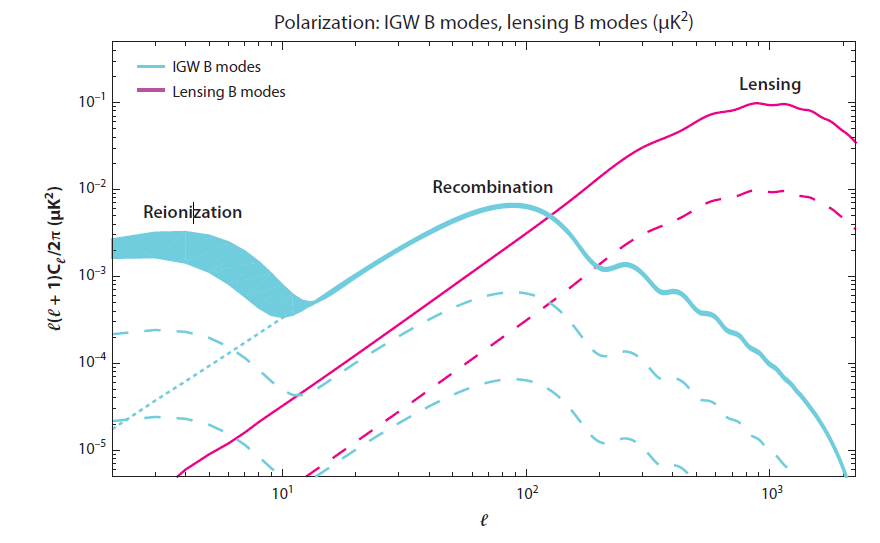
\includegraphics[width=\linewidth]{lensingfucksus.png}
  \caption{Polarisation power. Spectra are shown for primordial B modes with $r=\{0.1,0.01,0.001\}$ in cyan, and lensing induced B modes in magenta. The $\pm1\sigma$ uncertainity is due to the current constraint on $\kappa$, the optical depth to reionization is indicated for $r=0.1$. The cyan dotted line is the result with no reionization. a 90\% delensed signal is shown in dotted magenta. Plots generated using CAMB (lewis et al 2000)}
  \label{lensingisfucked}
\end{figure}

Given our precise measurements of most cosmological parameters from Planck 2015 [ref], and using the main results of this essay \ref{primordialBmodes} and (a full sky version of ) \ref{lensedBmodes}, \ref{lensingisfucked} demonstrates how large a problem lensing really is. We see the lensing contribution obscures IGW B modes at small scales, though for r sufficiently large: i.e. within roughly an order of magnitude of the upper bound, the recombination bump may may still stand out. Several experiments have confirmed detection of  these lensing B modes in the range $200<l<1500$. COUPLE REFERENCES FROM QBM. \\

\subsubsection{Delensing}

In the limit of small instrumental noise, the argest source of B-mode power on large angular scales is gravitational lensing. The lensed B-mode power spectrum $\tilde{C}^{BB}_l$ is roughly constant on large angular scales, and can thus be interpreted as an extra source of white noise. For instrumental noise levels falling below this white noise experiments will be lensing-limited: the limiting factor in constraining r will be the lensing B-mode. Delensing algorithms have been proposed [14, 15, 16] which statistically separate the gravitational wave and lensing B-mode signals, offering the prospect for reducing the noise floor and unlocking more modes for observation. These algorithms are based on a relatively simple idea: given information about noisy observed E modes, together with information about the lensing potential and therefore the deflection field, we can estimate the large-scale lensing B-mode and subtract it from the observed B-mode.\\

The required estimate for the defection field can be any probe of the universes matter distribution, and can be obtained externally or internally. External probes include galaxy surveys of the cosmic IR background. For illustration we discuss an example of an internal estimate in the next section, i.e. from the CMB itself.\\

Given an such an estimator $\hat{\psi}(\v{l})$, we may use the lensed E mode as a proxy for the unlensed E mode, and write, via taking the imaginary part of \ref{lensedEBmodes}

\begin{equation}
B^{\text{rec}}(\v{l}) = \finttwo{l_1} \v{l_1}\cdot(\v{l}-\v{l_1}) \tilde{E}(\v{l_1})\hat{\psi}(\v{l}-\v{l_1})\sin[2(\phi_\v{l_1}-\phi_\v{l})]
\end{equation} 

which we then subtract off of our observed B modes, getting a delensed mode:

\begin{equation}
B^{\text{delensed}}(\v{l}) = B^{\text{observed}}(\v{l}) - B^{\text{reconstructed}}(\v{l})
\end{equation}

\subsubsection{Lensing reconstruction}

The step we brushed under the rug above was the reconstruction of the lensing potential. Here we discuss the simplest such estimators, which have recently been used to create lensing mass maps over large portions of the sky by the ACT collaboration. \\

The idea here is that the unlensed CMB is statistically very simple - it is Gaussian, ie distinct fourier modes are statistically independent: $\langle X^*(\v{l})X(\v{l'})\rangle =0 \text{for} \v{l} \neq \v{l'}$. Lensing, being a non linear effect mixes these fourier modes: we saw above by the convolution theorem that  $\tilde{X}(\v{l})$ picks up contributions from all modes ${X}(\v{l_1}$ and $\phi(\v{l_2}$ with $\v{l_1}+\v{l_2}=\v{l}$. It thus contains information about the lensing potential.\\

Let us demonstrate this explicitly for the case of temperature pertubations. From the expression \ref{lensedtemp} we calculate the average over many CMB

\begin{equation}\begin{split}
\langle \tilde{\Theta}(\v{l})\tilde{\Theta}^*(\v{l}-\v{L})\rangle_{\Theta} &= \delta(\v{L})C_l^{\Theta\Theta} \finttwo{l_1}  \v{l_1}\cdot(\v{l}-\v{l_1})\psi(\v{l}-\v{l_1}) \langle \Theta(\v{l_1})\Theta^*(\v{l}-\v{L})\rangle \\
&\qquad + \v{l_1}\cdot(\v{l}-\v{L}-\v{l_1})\psi^*(\v{l}-\v{L}-\v{l_1}) \langle \Theta(\v{l})\Theta^*(\v{l_1})\rangle\\
&=\delta(\v{L})C_l^{\Theta\Theta} + [(\v{L}-\v{l})\cdot\v{L}C^{\Theta\Theta}_{|\v{l}-\v{L}|}+\v{l}\cdot\v{L}C_l^{\Theta\Theta}]\psi(\v{l})
\end{split}\end{equation}

and so the $\v{L}\neq 0 $ modes probe the lensing potential. To estimate the lensing potential we perform a weighted average of all off diagonal terms:

\begin{equation}
\hat{\psi}(\v{L}) = N(\v{L})\finttwo{l} \tilde{\Theta}(\v{l})\tilde{\Theta}^*(\v{l-L})g(\v{l},\v{L})
\end{equation}

where $g(\v{l},\v{L})$ is some weighting function. To be unbiased at lowest order we want $\langle \hat{\psi}(\v{L}) \rangle_\Theta = \psi(\v{L})$, which by the previous calculation gives:

\begin{equation}
N(\v{L})^{-1} = \finttwo{l} [(\v{L}-\v{l})\cdot\v{L}C^{\Theta\Theta}_{|\v{l}-\v{L}|}+\v{l}\cdot\v{L}C_l^{\Theta\Theta}]g(\v{l},\v{L})
\end{equation}

We now choose $g$ to maximise the signal to noise. One can compute the variance to zeroth order in $C_l^{\psi\psi}$ as $\langle| \hat{\psi}(\v{L})-\psi(\v{L})|^2 \rangle \approx 
\langle| \hat{\psi}(\v{L})|^2 \rangle$ which can be computed as:

\begin{equation}
\langle\hat{\psi}^*(\v{L}) \hat{\psi}(\v{L}) \rangle = \delta(\v{0})2N(\v{L})^2\finttwo{l}\tilde{C}_l^{tot}\tilde{C}_{|\v{l}-\v{L}|}^{tot}g(\v{l},\v{L})^2 + O(C_l^{\psi\psi})
\end{equation}

where $\tilde{C}_l^{tot} = \tilde{C}_l^{\Theta\Theta} + N_l$ is the total observed lensed + noise spectrum. By differentiating this variance with respect to g, we may minimize the variance via the choice

\begin{equation}
g(\v{l},\v{L}) = \frac{[(\v{L}-\v{l})\cdot\v{L}C^{\Theta\Theta}_{|\v{l}-\v{L}|}+\v{l}\cdot\v{L}C_l^{\Theta\Theta}]}{2\tilde{C}_l^{tot}\tilde{C}_{|\v{l}-\v{L}|}^{tot}}
\end{equation}

completing the construction of the minimum variance estimator. 

\begin{equation}
\hat{\psi}(\v{L}) = N(\v{l})\v{L}\cdot\finttwo{l} \frac{C_l^{\Theta\Theta}\tilde{\Theta}(\v{l})\tilde{\Theta}^(\v{L-l})}{\tilde{C}_l^{tot}\tilde{C}_{|\v{l}-\v{L}|}^{tot}}
\end{equation}

This allows us to estimate the lensing potential, to within some noise This has lowest order variance, or noise, given by


\begin{equation}
\delta(\v{0}) \langle |\hat{\psi}(\v{L})|^2 \rangle^{-1} =  N(\v{L})^{-1} = \finttwo{l}  \frac{[(\v{L}-\v{l})\cdot\v{L}C^{\Theta\Theta}_{|\v{l}-\v{L}|}+\v{l}\cdot\v{L}C_l^{\Theta\Theta}]^2}{2\tilde{C}_l^{tot}\tilde{C}_{|\v{l}-\v{L}|}^{tot}}
\end{equation}


We have constructed the estimator from solely the temperature field here. The polarisation fields also provide useful information and one can construct 6 minimum variance estimators out of the three fields: $\{TT, TE, TB, EE, EB, BB\}$, each with different normalisation and weight functions, which can be found in Hu and Otomoto. In practice, all 6 can be combined with minimum variance weighting to give a total minimum variance estimator, which is the approach taken in practice. This is a lot harder than presented here - one has to be careful with their statistics to ensure results obtained have quantifiably low noise to be able to make meaningful physics predictions.






















\section{Probing inflationary physics}

Inflation is a compelling solution of the homogeneity, flatness and monopole problems of the standard big bang cosmology. In addition, quantum fluctuations during inflation provide an elegant mechanism to seed future structure formation. The predictions of inflation: an adiabatic, nearly scale invariant spectrum of density pertubations match observations very closely. The B mode diagnostic is often termed to be a `smoking gun' for inflation: if detected it would provide very strong evidence for inflation, and give us significant insight into it's physics. In this chapter we firstly discuss why this first statement is true, and go on to discuss what additional constraining power a detection of primordial tensors would provide.

\subsection{Inflation Alternatives}

It is still up for debate as to whether inflation actually occurred, and a fair evaluation as to the status of inflation requires consideration of alternatives, which we briefly  review here. They are disfavoured for two reasons: Firstly, each invokes novel and not well understood physics to solve the three problems with the big bang cosmology. These theoretical issues need addressing before the models can be regarded as compelling alternatives to inflation. Secondly, most predict negligible primordial tensor perturbations. This strengthens the constraining power of the B mode diagnostic: a detection of primordial tensor pertubations has the power to rule out some of these other models completely. \\

\textbf{Ekpyrotic/Cyclic Cosmology}: The Ekpyrotic cosmology speculates an initial cold beginning and phase of slow contraction, followed by a bounce leading to the standard decelerating FLRW cosmology. Despite being entirely opposite to the idea of inflation, the model claims to be equally succesfull in solving the flatness and homogeneity problems. It's cyclic extension involves our current expansion to be followed by a contracting ekpyrotic phase, leading to a new hot Big Bang phase, continuing ad infinitum. The model has several theoretical issues: The bouncing phase requires a violation of the null energy condition, usually associated with catastrophic instabilities, and so has been hard to model consistently in a UV complete theory. A simple model is analogous to inflation, with a scalar field, instead rolling fast down its potential. One expects therefore the curvature perturbation then to have a very blue spectrum, in stark contrast with the observed near scale invariance. Similarly the tensor spectrum is highly blue, resulting in exponentially small primordial gravitational wave amplitudes for observable modes. Encouragingly we may rule this out with a detection then of B modes.\\


\textbf{String Gas Cosmology} This postulates an initially hot dense state similar to the standard big bang cosmology. All dimensions are taken to be compact and at the string scale, with the scale inversion symettry $R\rightarrow 1/R$ fundamental to string theory. This model predicts the decompactification of three spatial dimensions, leaving the remaining dimensions stably compact, which combined with the natural hot initial state of the universe makes it appealing. The theoretical issue heres are the need for seemingly large amount of fine tuning required, as well as issues with reheating. Recent work has claimed the model is capable of generating nearly scale invariant scalar pertubations and a blue tilted spectrum of tensor pertubations, agreeing with observations thus far but distinctly different to inflation. A measurement of $n_t$ however is far in the future.\\

\textbf{Pre-Big Bang Cosmology} Another string-theoretic model, this begins with a cold empty universe with zero curvature. Quantum fluctuations druve the universe into a scalar field driven super inflation, during which the expansion rate is increasing. This continues until the expansion rate reaches the string scale, at which point string-y corrections are required on the effective field theory description. These cause the expansion rate to be capped at a rate near the string scale, after which the universe reheats and enters radiation domination. Theoretical issues here involving the transition to radiation domination have slowed progress, and no solution to the horizon or flatness problems exist yet. This model therefore is not yet mature enough to be considered a worthy alternative to inflation








Given the large number of inflation models, even within the SFSR regime, that exist in the literature, it is useful to work model independently. We'll describe some ifnromation we can gather:

\subsection{The energy scale of inflation}


In the slow roll approximation, the tensor power spectrum depends only on the hubble rate during inflation, which in SFSR models can be related to the inflaton potential via $3H^2\Mp^2\approx V$. The scalar power spectrum depends both on the hubble rate, as well as the slow roll parameter $\epsilon$, which is directly related to the scalar to tensor ratio $r$. Given these, we may compute the energy scale of inflation. Working at the pivot scale $k_* = 0.05Mpc^{-1}$

\begin{equation}
\Delta^2_{\mathcal{s}}\approx \frac{V}{24\pi^2\epsilon\Mp^4}
\end{equation}

Current measurements [QBM -> PLANCK] give $ A_s \approx 2.2\times10^{-9}$. Making use of $r\approx 16\epsilon$, and $\Mp \approx 2.43\times 10^{18} GeV$ we learn

\begin{equation}\begin{split}
V=24\pi^2A_s\frac{r}{16}\Mp^4 \Rightarrow V^{1/4} &\approx 3.22\times10^{16}\text{GeV}r_*^{1/4}\\
&= 1.04\times10^{16}\text{GeV}(\frac{r_*}{0.01})^{1/4} \leq 1.75\times10^{16}\text{GeV}
\end{split}\end{equation}

where the inequality comes from the current bound $r_*\leq 0.1$ provided by a lack of detection of a tensor power spectrum to a given sensitivity. A detectably large tensor amplitude would be very good evidence for inflation, and demonstrate a tremendously high new fundamental energy scale in physics - comparable to that of Grand Unified Theories. Let us not understate this - this will be exceedingly important for the high energy physics community, a result we have no hope to gain significant insight into via terrestrial collider experiments. 


\subsection{Field excursion}

As before, combining the scalar and tensor power spectrum gives information about $\epsilon$, which in the slow roll regime contains information about the background evolution of the field. In particular, recalling our previous calculation \ref{efolds} we can compute the "field excursion" of the inflaton field in planck units:

\begin{equation}\begin{split}
N(t) &=  \int_{\phi(t)}^{\phi_{end}} \frac{d\phi}{\sqrt{2\epsilon}\Mp}\\
\Rightarrow dN&=\frac{d\phi}{\sqrt{2\epsilon}\Mp}\\
\Rightarrow \frac{\Delta \phi}{\Mp} &= \int_0^N \sqrt{2\epsilon} dN = \int_0^N \sqrt{r/8} dN 
\end{split}\end{equation}

Now recall each mode inflates do a slightly different degree depending on when it leaves the horizon: we can apply this formula to the pivot scale mode $k_*$ to learn 

\begin{equation}
\frac{\Delta \phi}{\Mp} =  \int_0^{N_*} \sqrt{\frac{r(N)}{8}} dN  = (\frac{r_*}{8})^\half N_{\text{eff}}
\end{equation}

where $N_eff$ is model dependent and given by

\begin{equation}
\int_0^{N_*}(\frac{r(N)}{r_*})^\half dN
\end{equation}


In slow roll inflation $r$ is approximately constant, but depends slightly on $N$, precisely because $\epsilon$ varies slightly during inflation. In most models, we can take $\epsilon$ to increase over time monotonically, and so $r$ is monotonically increasing with $N$ and so

\begin{equation}
\frac{\Delta \phi}{\Mp} > \sqrt{r_*/8}N_* > (\frac{r}{0.01})^{1/2}
\end{equation}

where the second inequality comes from a conservative lower limit on $N_* > 30$. This is a lot lower than the requirement of about 55 e folds of inflation we require to solve the horizon and flatness problems. Nevertheless, we see can seperate inflation models into two (vaguely) distinct classes, depending on if $r\lessapprox 0.01$ or $r\gtrapprox 0.01$, known as small and large field models. This is the Lyth bound. \\


\begin{figure}[h]
  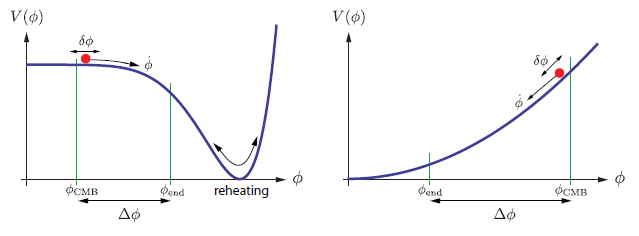
\includegraphics[width=\linewidth]{smalllargefield.png}
  \caption{Examples of typical small (left) and large (right) field models, with field excursion shown.}
\end{figure}

While both small and large field models are challenging to construct consistently, and require some degree of fine tuning, large field models prove more difficult. Suppose we expand the inflaton potential in a SFSR model as 

\begin{equation}
V(\phi) = \half m^2\phi^2 + \sum_{p=3}^\infty \lambda_p(\frac{\phi}{\Mp})^p
\end{equation}

We can fine tune $\lambda_p$ such that at any $\phi$, $\epsilon, \eta << 1$, though these coefficients are expected to receive quantum corrections $\Delta\phi_p(\\phi)$, which generically will be of order unity in superplanckian field ranges, and so are expected in large field inflation. It is hard to see inflation being maintained for sufficiently many e folds as $\epsilon, \eta << 1$ would likely not be preserved of this full range. \\

Again, a detection (or lack thereof) of $r$ in upcoming CMB experiments, with forecasted sensitivity $r\approx 10^{-3}$, would have far reaching implications for inflationary model building. It would be able to definitively either validate or rule out such large field models, and further, given the energy scales at play, would give a first observational constraint on potential quantum-gravity unified theories.

\subsection{Model Dependent Results}

Having worked fairly model independently thus far, we give some examples of particular SFSR models. From the shape of the potential $V$ and the number of e folds of inflation $N_*$ at some pivot scale we may derive expressions for the two observational quantities of interest $n_s$ and $r$. 


\textbf{Large field models} We demonstrate this calculation described above in the case of a power law potential

\begin{equation}
V(\phi) = \half m^{4-\alpha}\phi^\alpha
\end{equation}

for m a mass parameter required to give the potential the correct mass dimension. We may compute 

\begin{equation}
\epsilon_V = \frac{\Mp^2\alpha^2}{2\phi^2}
\end{equation}

and therefore

\begin{equation}
\begin{split}
N &= \int_{\phi_e}^\phi \frac{d\phi}{\Mp}\frac{1}{\sqrt{2\epsilon}} \\
&= \frac{1}{2\Mp^2}(\phi^2-\phi^2_e)\\
&= \frac{\alpha}{4}(\frac{1}{\epsilon-1}
\end{split}
\end{equation}

using $\epsilon(\phi_e)=1$. This gives $\epsilon_V \approx \frac{\alpha}{4N}$ to first order in slow roll parameters. Using this, one calculates $\eta_V=\frac{\alpha-1}{2N}$. Finally we obtain

\begin{equation}
n_s-1 = -\frac{2+\alpha}{2N} \qquad r=\frac{4\alpha}{N}
\end{equation}

We may break the degeneracy by using the Planck best fit value of $n_s=0.968$ to express $N=N(\alpha)$. We can extract the energy scale at the end of inflation as  $V(\phi_e)=m^{4-\alpha}\frac{\alpha\Mp}{\sqrt{2}}^\alpha/2$, and also infer the field excursion.\\

Other large field models include natural inflation, motivated by axions

\begin{equation}
V(\phi) \propto 1+\cos\frac{\phi}{f}
\end{equation}

where f is some periodic function.

\textbf{Small field models} The hilltop model is a fairly typical looking small-field model, with

\begin{equation}
V(\phi) \propto 1-(\frac{\phi}{\mu})^p 
\end{equation}

for $p>2$, ($p=2$ turns out to be large field). This predicts $n_s-1 \approx \frac{-2}{N}\frac{p-1}{p-2}$ and an upper limit on $r\lesssim 8\frac{p}{N(p-2)}(\frac{8\pi}{Np(p-2P})^{p/(p-2)}$.\\


One can rule out certain models completely by making use of current measurements, as shown in figure \ref{inflationconstraints}. 

\begin{figure}[h]
  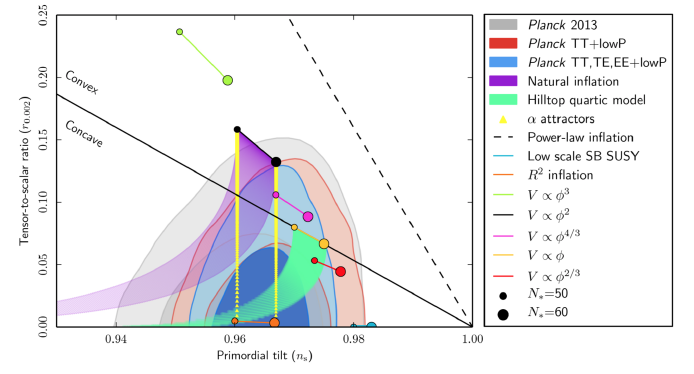
\includegraphics[width=\linewidth]{modeldepconstraints.png}
  \caption{Current constraints on $n_s$ and $r$ by the Planck 2013 and more recent Planck 2015 data release (REF) The predictions for $N_*=50$ and $N_*=60$ from a variety of different inflationary models are shown. Concave and convex refer to the sign of the second derivative of the inflaton potential. `lowP' refers to data from the large-scale WMAP polarization survey}
\label{inflationconstraints}  
\end{figure}

For progress to be made we must collapse the current large range of allowed $r$ values. A detection of $r$ would do so significantly.

\begin{figure}[h]
  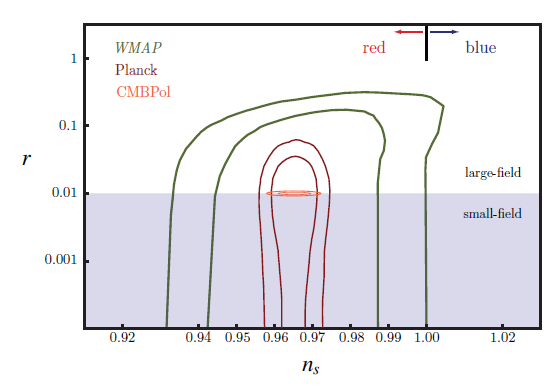
\includegraphics[width=\linewidth]{forecastconstraints.png}
  \caption{Forecasted constraints on $n_s$ and $r$ by future CMB experiments are far greater, with much greater sensitivity on r - shown here for a measured value $r=0.01$ }
\label{inflationconstraints}  
\end{figure}



































\appendix

\section{Properties of spin-weighted functions}
We list here the properties of spin-weighted functions we'll need. For each integer spin s separately, there exist a basis of spin-weighted functions $_sY_{lm}$ on the sphere, satisfying the same orthogonality and completeness relations as regular spherical harmonics

\begin{equation}
\begin{split}
\int_0^{2\pi} d\phi \int_{-1}^{1} d(\cos{\theta}) {}_sY_{l'm'}^*(\theta,\phi){}_sY_{lm}(\theta,\phi) = \delta_{ll'}\delta{mm'} \\
\sum_{lm} {}_sY_{lm}^*(\theta,\phi){}_sY_{lm}(\theta',\phi')=\delta(\phi-\phi')\delta(\theta-\theta')
\end{split}
\end{equation}

There also exist spin raising ($\sr$) and spin lowering ($\sl$) operators, which raise or lower the spin weight of a function $_sf(\theta,\phi)$ by 1, with explicit expression given by

\begin{equation}\begin{split}
\sr {}_sf(\theta, \phi) &= -\sin^s{\theta}[\partial_\theta+i\csc{\theta}\partial_\phi]\sin^{-s}{\theta}{}_sf(\theta, \phi)\\
\sl {}_sf(\theta, \phi) &= -\sin^{-s}{\theta}[\partial_\theta-i\csc{\theta}\partial_\phi]\sin^{s}{\theta}{}_sf(\theta, \phi)
\label{explicitspinraiselower}
\end{split}\end{equation}

Polarisation quantities are spin $\pm 2$, which we often wish to raise or lower to spin 0. In the case where we have ${}_{\pm2}f(\mu,\phi)$ satisfying $\partial_\phi{}f=imf$ we can derive the following forms of the $\sr^2$ and $\sl^2$ operators

\begin{equation}\begin{split}
\sl^2{}_2f(\mu, \phi) &= (-\partial_\mu+\frac{m}{1+\mu^2})^2[(1-\mu^2)_2f(\mu,\phi)]\\
\sr^2{}_{-2}f(\mu, \phi) &= (-\partial_\mu-\frac{m}{1-\mu^2})^2[(1-\mu^2)_{-2}f(\mu,\phi)]
\label{+-2}
\end{split}\end{equation}

The spin weighted spherical harmonics $_sY_{lm}$ are related to the standard spherical harmonics $Y_lm$ by the relations:

\begin{equation}
_sY_{lm} = 
\begin{cases}
[\frac{(l-s)!}{(l+s)!}]^{1/2}\sr^s Y_{lm} & 0\leq s\leq l\\
[\frac{(l-s)!}{(l+s)!}]^{1/2}(-1)^s\sl^s Y_{lm} & -l\leq s\leq 0
\end{cases}
\end{equation}

Finally the following properties are useful

\begin{equation}\begin{split}
{}_sY_{lm}^* &= (-1)^s {}_{-s}Y_{l,-m}\\
\sr {}_sY_{lm} &= \sqrt{(l-s)(l+s+1)}{}_{s+1}Y_{l,m}\\
\sl {}_sY_{lm} &= \sqrt{(l-s)(l-s+1)}{}_{s-1}Y_{l,m}\\
\sl\sr {}_sY_{lm} &= -(l-s)(l+s+1){}_{s}Y_{l,m}
\label{propertiesofspin}
\end{split}\end{equation}

\section{Essay Description}
Our most promising theory for the early universe involves a phase of cosmic inflation, which not only rapidly expands and flattens the universe, but also generates the primordial density perturbations from quantum fluctuations in the inflaton field. While we have good evidence for inflation, e.g. from the Gaussianity, adiabaticity and near-scale invariance of the scalar density perturbations, one prediction of inflation has not yet been found: many inflationary models produce a stochastic background of primordial gravitational waves. A detection of this background would not only provide a definitive confirmation of inflation, but could also give new insights into the microphysics of inflation and, more broadly, physics at the highest energies.\\

The best current way of finding this gravitational wave background is to search for a characteristic pattern in the polarization of the Cosmic Microwave Background (CMB), the B-mode polarization. This essay should explain the physics underlying the search for this B-mode polarization pattern, which is currently a major area of research in cosmology.
The essay should first review the calculation of the gravitational wave background produced
by standard single-field slow-roll inflation, a standard result described in past Part III lecture notes as well as a comprehensive review of the field (Kamionkowski \& Kovetz 2016, henceforth KK16). The essay should also explain why the strength of the gravitational wave background(together with the scalar spectral index) can provide powerful constraints on the properties of inflation, such as the potential shape, energy scale, and field excursion (CMB-S4 2016, KK16).\\

Drawing on KK16, CMB-S4 2016, past lecture notes and other resources, the essay should provide a (brief) review of the basics of CMB polarization, describe what the CMB B-mode polarization is, and explain why it is a powerful probe of inflationary gravitational waves.\\

The remaining parts of the essay can, to some extent, be tailored to the student’s interests. One option is to explain in detail the major observational challenges in B-mode searches for inflationary gravitational waves, discussing the problems of foregrounds (Bicep/Keck/Planck 2015) and gravitational lensing as well as mitigation methods such as multifrequency cleaning and delensing (Smith et al. 2012). Another option is to focus more on the theoretical background, describing in detail different classes of inflationary models and what these generically predict for B-mode polarization (CMB-S4 2016 and references therein). Students may also discuss a combination of both observational and theoretical aspects.\\

\textbf{Relevant Courses}\\

\textit{Essential}: Cosmology\\

\textit{Useful}: Advanced Cosmology, Quantum Field Theory, General Relativity\\

\textbf{References}
\begin{enumerate}[label={[\arabic*]}]
\item {Kamionkowski, M. \& Kovetz, E. D. 2016, Annual Review of Astronomy and Astrophysics,
54, 227}
\item {CMB-S4 Science Book 2016, arXiv:1610.02743 (mainly chapter 2)}
\item {BICEP/Keck/Planck 2015, arXiv:1502.00612, Phys. Rev. Lett. 141 101301}
\item {Smith, K. M. et al. 2012, arXiv:1010.0048, JCAP, 06 014}
\item {Baumann, D., lecture notes: http://www.damtp.cam.ac.uk/user/db275/Cosmology/Lectures.pdf}
\end{enumerate}





\section{The Boltzmann Equation}

this section might have to go\\


Now that we understand how to describe the relevant quantities on the sphere, we must understand the physics describing their evolution in the early universe, at the epoch of recombination. We use the formalism of distribution functions, and the boltzmann equation, only slightly extending the treatment described in lectures. There are four distribution functions to keep track of now, one for each of the Stokes parameters. We'll make concrete the claim that we may neglect the V stokes parameter, by showing it doesn't evolve from its primordial black body $V=0$ distribution. We'll first derive the Liouville equation, the left hand side of the Boltzmann equation, describing the evolution of the phase space distribution without the presence of a collision term. We'll omit deriving the collision term for Thomson scattering in detail, as the calculation is rather long, but a full discussion may be found in [], on which much of this section is based, although some different conventions are used: notably we use conformal time, and have swapped the newtonian potentials.

We seek to understand both scalar and tensor pertubations to a background FLRW spacetime. We neglect vector pertubations, which decay and are unimportant, unless sourced continuously, by topological defects for example. We use the Newtonian gauge form of the perturbed metric, and work to linear order in pertubations throughout.

\begin{equation}
ds^2 = a^2(\tau) [-(1+2\Psi)d\tau^2 + ((1-2\Phi)\delta_{ij} +h_{ij})dx^idx^j]
\label{perturbmetric}
\end{equation}

where the newtonian potentials are $\Phi$ and $\Psi$ and the metric pertubations $h_{ij}$ are transverse and traceless. 


Photons are described by space time coordinate $x^\mu$ and four momentum $p^\mu=\frac{dx^\mu}{d\lambda}$, and are null

\begin{equation}\begin{split}
g_{\mu\nu}p^\mu p^\nu&=0\\
-a^2(1+2\Psi)((p^0)^2 + p^2) = 0\\
\Rightarrow p^0 = \frac{p}{a}(1-\Psi)
\end{split}\end{equation}

We have introduced $p^2=g_{ij}p^ip^j$, the physical photon momentum. We now factorise the spatial part of the metric into an amplitude an angular part $p^i = C\hat{p}^i$, such that $\delta_{ij}\hat{p}^i\hat{p}^j=1$ with $C$ being determines by the constraint:

\begin{equation}
a^2((1-2\Phi)\delta_{ij}+h_{ij})p^ip^j = p^2 \Rightarrow C=\frac{p}{a}(1+\Phi-\half h_ij\hat{p}^i\hat{p}^j)
\end{equation}

so the photon 4 momentum may be written as 

\begin{equation}
p^\mu = \frac{p}{a}(1-\Psi, (1+\Phi-\half h_{jk}\hat{p}^j\hat{p}^k)\hat{p}^i))
\end{equation}

The Liouville equation for a distribution $f=f(\tau, x^\mu, p^\mu)$ as

\begin{equation}
\frac{df}{d\tau} = \frac{\partial f}{\partial\tau} + \frac{\partial f}{\partial x^i} \frac{dx^i}{d\tau} + \frac{\partial f}{\partial p} \frac{dp}{d\tau} + \frac{\partial f}{partial\hat{p}^i} \frac{d\hat{p}^i}{d\tau}  = 0
\label{Liouville}
\end{equation}

We wish to evaluate this to 0'th and 1'st order. It can be shown the final term is second order, as both $\frac{\partial f}{partial\hat{p}^i}$ and  $\frac{d\hat{p}^i}{d\tau}$ are first order quantities. Physically, the first is because the background distribution is isotropic, and the second is since the unperturbed geodesics are straight lines. \\

The $\frac{dx^i}{d\tau}$ term is easily computed:

\begin{equation}
\frac{dx^i}{d\tau} = \frac{dx^i}{d\lambda}\frac{d\lambda}{d\tau} = \frac{p^i}{p^0} = (1+\Phi+\Psi-\half h_jk\hat{p}^j\hat{p}^k)\hat{p}^i
\end{equation}

whereas $\frac{dp}{d\tau}$ requires more work - it describes the evolution of the photon energy, which is described by the geodesic equation. Since we are working to linear order here, the scalar and tensor pertubation contributions decouple, and we can calculate the contribution of each separately. After a slightly tedious calculation we arrive at 

include steps??? got them on a piece of paper somewhere

\begin{equation}
\frac{dp}{d\tau} = p (\Phi' - \hat{p}^i\frac{\partial \Psi}{\partial x^i} -\half h_ij\hat{p}^i\hat{p}^j -\mathcal{H})
\end{equation}

That's all we need. We may decompose any distribution to linear order as $f(x^\mu, p^\mu) = f^{(0)}(p,\tau) + f^{(1)}(\v{x},p,\hat{p}^i,\tau)$. Plugging this, and the above results into \ref{Liouville} we get the following 0'th and 1'st order equations

\begin{equation}\begin{split}
\frac{\partial f^{(0)}}{d\tau} - p\mathcal{H}\frac{\partial f^{(0)}}{dp} &=0\\
\frac{\partial f^{(1)}}{d\tau} + \hat{p}^i\frac{\partial f^{(1)}}{dx^i} - p\mathcal{H}\frac{\partial f^{(1)}}{dp} +p\frac{\partial f^{(0)}}{dp}(\frac{\partial\Phi}{d\tau}-\hat{p}^i\frac{\partial \Psi}{dx^i}-\half \frac{\partial h_{ij}}{d\tau}\hat{p}^i\hat{p}^j) &=0
\end{split}\end{equation}

The zeroth order equation has solution $f^{(0)}(k,\tau) = f^{(0)}(ka)$, explaining the background uniform redshift, as expected. We can fourier transform over the spartial $\v{x}$ dependence of the first order equation, and reintroduce the collision term, obtaining $f = f^{(1)} = f^{(1)}(\v{k}, p, \hat{p}^i, \tau)$

\begin{equation}
f^{(1)'} + ik\mu f^{(1)}-\mathcal{H}p\frac{\partial f^{(1)}}{\partial p} - \frac{\partial f^{(0)}}{\partial k} [ \Phi ' - \Psi ' + ik\mu \Phi + \half h_{ij}'\hat{p}^i\hat{p}^j] = 
C
\end{equation}
where we have introduced $\mu = \unit{k} \cdot \unit{p}$, the angle cosine between photon propagation and fourier mode.

C represents the collision term. For scalar pertubations, it contains source terms proportional to $\unit{p}\cdot\v{v_e}$, for $v_e$ the photon velocity. However, scalar perturbations produce velocities $\v{v} \propto \v{k}$, so we may choose spherical coordinates for $\unit{p}$ to be aligned with $v{k}$. In this case  $f^{(1)}(\v{k}, p, \hat{p}^i, \tau) = f^{(1)}(\v{k}, p, \mu, \tau)$, and is manifestly invariant of $\theta$.

Tensor pertubations do depend on $\phi$. Neglecting any electron velocity arising from tensor pertubations, all the $\phi$ dependence is characterised by the tensor pertubation in the boltzmann equation:

\begin{equation}
h_{ij}'(\v{k},\tau)\hat{p}^i\hat{p}^j = \hat{p}^i\hat{p}^j (h^{+'}(\vec{k},\tau)e_{ij}^+(\vec{k}) + h^{\times'}(\vec{k},\tau)e_{ij}^\times(\vec{k})
\end{equation}

Choosing spherical coordinates with z axis aligned with $\v{k}$, we choose simple polarisation vectors $e^+_{xx}=-e^+_{yy}=1$ and $e^\times_{xy}=e^\times{yx}=1$ with other components 0. From this we calculate using $\hat{k}^i = (\sin\theta\cos\phi, \sin\theta\sin\phi, \cos\phi)$

\begin{equation}\begin{split}
\hat{p}^i\hat{p}^je_{ij}^+ &= \sin^2{\theta}\cos{2\phi} \\
\hat{p}^i\hat{p}^je_{ij}^\times &= \sin^2{\theta}\sin{2\phi}
\end{split}\end{equation}

and so we may write 

\begin{equation}
f^{(1)}(\v{k}, p, \hat{p}^i, \tau) = f^{(1)}(\v{k}, p, \mu, \tau)\cos{2\phi}
\end{equation}

for a + polarized wave


\begin{equation}
f^{(1)}(\v{k}, p, \hat{p}^i, \tau) = f^{(1)}(\v{k}, p, \mu, \tau)\sin{2\phi}
\end{equation}

for a x polarized wave


\section{Old Inflation Chapter}

Inflation is a brief, but very important, period of accelerated expansion in the very early universe, first proposed by [Guth 1981]. It was initially motivated by three problems with the previous standard big bang cosmology, namely the flatness problem (why was the ratio of energy density and critical density so close to unity), the monopole problem, and the horizon problem (why are seemingly casually disconnected regions of the CMB at the same temperature to very high accuracy). Since the birth of the idea, it has become the leading paradigm to the early universe, in part because it provides a quantum mechanical mechanism of generating the primordial density perturbations seeding cosmological evolution. In this chapter we quickly review some important features of inflation.

\subsection{Inflation Basics}

A flat, homogeneous and isotropic universe is described by the Friedmann–Lemaître–Robertson–Walker (FLRW) metric, which in our sign convention takes form

\begin{equation}
\label{FLRW}
ds^2 = - dt^2 + a^2(t)d\v{x}^2 = a^2(\tau)(-d\tau^2+d\v{x}^2)
\end{equation}

and, assuming General Relativity, obeys the Einstein equation $G_{ab} = \frac{1}{\Mp^2} T_{ab}$, sourced by a perfect fluid with energy momentum tensor $T_{ab}$, which by homogeneity and isotropy must take form

\begin{equation}
\label{densityandpressure}
T^0_0 = - \rho(t) \quad T^0_i = 0 \quad T^i_j = P(t)\delta^i_j
\end{equation}

where we  identify $\rho(t)$ as the total energy density and $P(t)$ as the total pressure, ie summed over all fluid components. For our purposes, we will consider one component, the inflaton field, to dominate.  Substituting \ref{FLRW} and \ref{densityandpressure} into the Einstein Equation we obtain the Friedmann equations

\begin{equation}
H^2 = (\frac{\dot{a}}{a})^2 = \frac{1}{3\Mp^2}\rho
\tag{F1}
\label{F1}
\end{equation}
\begin{equation}
\frac{\ddot{a}}{a} = -\frac{1}{6\Mp^2}(\rho + 3P)
\tag{F2}
\label{F2}
\end{equation}

The condition for inflation to occur is \textit{accelerated expansion}, ie $\ddot{a} >0$. Recall the definition of the first hubble slow roll parameter 

\begin{equation}
\label{epsilon}
\epsilon := -\frac{\dot{H}}{H^2} = -\frac{d\ln{H}}{d\ln{a}} = \frac{3}{2}(1+\frac{P}{\rho})
\end{equation}

where the last inequality follows from the Friedmann Equations. We find $\ddot{a} >0$ is equivalent to $\epsilon<1$ and to the condition on the equation of state parameter $\omega=P/\rho < -1/3$.\\ 

In order to solve the horizon problem we require inflation to persist for a relatively long duration of time (~60 e-folds), so $\epsilon$ to must remain small. We parametrise how quickly $\epsilon$ changes in the second hubble slow roll parameter 

\begin{equation}
\eta = -\frac{\dot{\epsilon}}{H\epsilon} = -\frac{d\ln{\epsilon}}{d\ln{a}}
\end{equation}

\subsection{Single Scalar Field Dynamics}

The simplest class of inflation models are those consisting of a single scalar field, slowly rolling down its potential. These postulate the existence of a scalar ``inflation'' field $\phi(t,\v{x})$ with lagrangian density $\mathcal{L} = -\half \partial^\mu \phi \partial_\mu \phi - V(\phi)$ and energy momentum tensor $T_{\mu\nu}= \partial_\mu \phi \partial_\nu \phi + g_{\mu\nu}\mathcal{L}$. \\

Here we consider the classical background evolution, ie take $\phi(t,\v{x}) = \bphi(t)$. There is of course no reason why the field should not also fluctuate spatially, which we consider in the next section. From \ref{densityandpressure} we see that 


SOME MISTAKE HERE OR IN PREVIOUS DEF
\begin{equation}\begin{split}
\rho_\phi &=-T^0_0 = \half \dot{\bphi}^2+V(\bphi)\\
P_\phi&=\frac{1}{3}T^i_i = \half \dot{\bphi}^2-V(\bphi)
\end{split}\end{equation}

Inserting these into the Friedmann equations we get the Klein Gordon Equation

\begin{equation}
\tag{KG}
\label{KG}
\ddot{\bphi}+3H\dot{\bphi}=-V_{,\phi}
\end{equation}

We also find that by \ref{epsilon} that 

\begin{equation}
\epsilon = \frac{1}{\Mp^2}\frac{\half\dot{\bphi^2}}{H^2} < 1
\end{equation}

\subsection{Slow Roll}

The slow roll approximation postulates the kinetic energy and acceleration of the background field is much smaller than its potential energy, which can be encapsulated in terms of our slow roll parameters as $(\epsilon, \eta << 1)$. In this approximation we get by \ref{F1} and \ref{KG} 

\begin{equation}\begin{split}
H^2 &\approx \frac{V}{3\Mp^2} \\
3H\dot{\bphi} &\approx -V_{,\phi}
\end{split}\end{equation}

from which we see 

\begin{equation}
\epsilon \approx \half\Mp^2 (\frac{V'}{V})^2 := \epsilon_V
\end{equation}

where we have defined the first \textit{potential} slow roll parameter. We can anologously define a second potential slow roll parameter via

\begin{equation}
\eta_V = \Mp^2 \frac{V''}{V} \approx 2\epsilon - \half\eta
\end{equation}

From here we may calculate the number of e folds of inflation from some time $t$ until the end of inflation. 

\begin{equation}
N(t) := \ln{\frac{a(t_{end})}{a(t)}} = \int_a^{a(t)} d(\ln{a}) = \int_t^{t_{end}} Hdt = \int_{\bphi(t)}^{\bphi_{end}} \frac{d\bphi}{\sqrt{2\epsilon_V}\Mp}
\label{efolds}
\end{equation}

using $Hdt=\frac{H}{\dot{\bphi}}d\bphi=\frac{d\bphi}{\sqrt{2\epsilon_V}\Mp}$

\subsection{Quantum Fluctuations to $\phi$}

If the inflaton can vary in time, it can also vary in space. The discussion here follows [Baumann]. We consider pertubations over a background

\begin{equation}
\phi(\v{x},\tau) = \bphi(\tau) + \frac{f(\tau, \v{x})}{a(\tau)}
\label{phiexpand}
\end{equation}

We begin with the action for the inflaton, minimally coupled to the metric.

\begin{equation}
S =\int d\tau d^3x \mathcal{L}  =  \int d\tau d^3x \sqrt{-g} (-\half g^{\mu \nu}\partial_\mu \phi\partial_\nu \phi - V(\phi)  
\end{equation}

Plugging in the unperturbed FLRW metric we get 


\begin{equation}
S = \int d\tau d^3x \mathcal{L}  = \int d\tau d^3x \half a^2 [(\phi ' )^2 -(\nabla \phi)^2]-a^4V(\phi)
\label{scalarfieldaction}
\end{equation}

We now plug in \ref{phiexpand} and expand to 2nd order in $f$. The first order piece just gives the Klein Gordon for the background field (in conformal time), as expected. The second order piece gives

\begin{equation}
S^{(2)} = \half \int d\tau d^3x (f')^2 - (\nabla f)^2 + (\frac{a''}{a}-a^2V'')f^2
\end{equation}

after integrating by parts and making use of \ref{F2} in conformal time. In the slow roll approximation we may drop the potential term since it is slow roll suppressed compared to the other terms.

and so 

\begin{equation}
S^{(2)} \approx \half \int d\tau d^3x (f')^2 - (\nabla f)^2 + \frac{a''}{a}f^2
\end{equation}

Note since we have dropped the potential entirely, this is just the second order action for a massless scalar field. Integrating by parts and demanding $S^{(2)}=0$ gives the Muhkanov Sasaki equation, which we can write in real or fourier space:

\begin{equation}\begin{split}
f''-\nabla^2f-\frac{a''}{a}f &= 0 \\
\Leftrightarrow f''_{\v{k}} + (k^2-\frac{a''}{a})f_{\v{k}} &= 0
\label{MS}
\end{split}\end{equation}

We treat these perturbations $f$ quantum mechanically, and so require the techniques of QFT on curved spacetimes. We'll outline the key steps in quantising this system.\\

The conjugate momentum to $f$ is $\pi(\tau, \v{x}) =  \frac{\partial \mathcal{L}}{\partial f'} = f'$ using \ref{scalarfieldaction}. We promote these to operators $\hat{f}(\tau, \v{x})$ and $\hat{\pi}(\tau, \v{x})$ satisfying equal time commutation relations which read in real and fourier space:

\begin{equation}\begin{split}
[\hat{f}(\tau, \v{x}), \hat{\pi}(\tau, \v{x'}] &= i\delta(\v{x}-\v{x'}) \\
[\hat{f}_{\v{k}}(\tau), \hat{\pi}_{\v{k'}}(\tau)] &= (2\pi)^3i\delta(\v{k}+\v{k'})
\end{split}\end{equation}

We mode expand $\hat{f}_{\v{k}}(\tau) = f_k(\tau)\ann{k}+f_k^*(\tau)\cre{k}$, demanding the modefunctions $f_k(\tau)$ and $f_k^*(\tau)$ are two linearly independent solutions of the Muhkanov-Sasaki equation. Substituting into the commutation relations we get 

\begin{equation}
W[f_k,f_k^*]\times[\ann{k}, \cre{k}] = (2\pi)^3\delta(\v{k}+\v{k'})
\end{equation}

which after normalising the Wronskian to 1 gives the usual commutator of annhilation and creation operators

\begin{equation}
[\ann{k}, \cre{k}] = (2\pi)^3\delta(\v{k}+\v{k'})
\end{equation}

We can now define the Hilbert space as the usual Fock space formed by unions of n particle states obtained by applying n creation operators to the the vacuum, satisfying 

\begin{equation}
\ann{k}\vac =0 \qquad \forall \v{k}
\end{equation}

Note this doesn't completely fix the vacuum, since we have not yet fixed our mode functions. We construct the Bunch-Davies vacuum, by imposing the mode functions must be positive frequency \footnote{this is required for our hilbert space to only consist of positive norm states, and is a common requirement in many quantum field theories}, and also match the minkowski mode functions $f_k(\tau) \propto e^{\pm ik\tau}$ at early times, since at early times $\tau \rightarrow -\infty$

\begin{equation}
\ref{MS} \rightarrow  f''_{\v{k}} + (k^2)f_{\v{k}} = 0
\end{equation}

We further make the quasi-deSitter approximation, where H is constant and $a=-\frac{1}{H\tau}$, and so \ref{MS} becomes

\begin{equation}
f''_k + (k^2-\frac{2}{\tau^2})f_k = 0
\end{equation}

with general solution

\begin{equation}
f_k(\tau) = \alpha \frac{e^{-ik\tau}}{\sqrt{2k}}{(1-\frac{i}{k\tau}} + \beta \frac{e^{ik\tau}}{\sqrt{2k}}{(1+\frac{i}{k\tau}})
\end{equation}

which matches our initial condition for $\beta = 0$ and $\alpha=1$, giving the Bunch Davies mode function 

\begin{equation}
f_k(\tau) = \frac{e^{-ik\tau}}{\sqrt{2k}}{(1-\frac{i}{k\tau}})
\end{equation}

The key result of this section is the power spectrum of fluctuations, given by 

%We now have all we require to calcuate the spatial variance, or two point correlator $\varepsilon(0)$ of $f$ and therefore of $\delta \phi = f/a$. First recall the relevant definitions:
%
%the two point correlation function of a field f is given by at fixed (omitted) time $\tau$ by
%
%\begin{equation} 
%\varepsilon_f(\v{x})f(\v{y}) = <f(\v{x})f(\v{y})> = <0|f(\v{x}f(\v{y})|0>
%\end{equation}
%
%Assuming statistical homogeneity and isotropy, this depends only on $|\v{x}-\v{y}|$, and is related to the power spectrum:

\begin{equation}
\langle f_{\v{k}}f_{\v{k'}} \rangle = \langle 0|f_{\v{k}}f_{\v{k'}}|0\rangle =(2\pi)^3\delta(\v{k}+\v{k'})P_f(k)\
\end{equation}

%by
%
%\begin{equation}
%\varepsilon(r)=\varepsilon(\v{x},\v{x}+\v{r})=\fint{k} P_f(k)e^{i\v{k}\cdot\v{r}}
%\end{equation}


The power spectrum of our field is easily computed to be 

\begin{equation}
\langle f_{\v{k}}f_{\v{k'}}\rangle = \langle (f_k(\tau)\ann{k}+f_k^*(\tau)\cre{k})(f_k(\tau)\ann{k'}+f_k^*(\tau)\cre{k'}\rangle = |f_k|^2
\end{equation}

and so the dimensionless power spectra of interest are  

\begin{equation}\begin{split}
\Delta^2_f(k):=\frac{k^3}{2\pi^2}P_f(k) &= \frac{k^3}{2\pi^2}|f_k|^2\\
\Rightarrow \Delta^2_{\delta\phi}(k) &=\frac{k^3}{2\pi^2a^2}|f_k|^2\\
&=\frac{k^2}{4\pi^2a^2}(1+\frac{1}{k^2\tau^2})\\
&=(\frac{H}{2\pi})^2(1+\frac{k^2}{a^2H^2} \text{using $a=\frac{-1}{H\tau}$}\\
&\rightarrow \frac{H}{2\pi})^2 \text{on superhorizon scales $k<<\mathcal{H}$}
\label{inflatonpower}
\end{split}\end{equation}

We approximate the power spectrum at horizon crossing to be 

\begin{equation}
\Delta^2_{\delta\phi}(k) \approx (\frac{H}{2\pi})^2\rvert_{k=aH}
\end{equation}

We will return to this result later.

































\acknowledgments

This is the most common positions for acknowledgments. A macro is
available to maintain the same layout and spelling of the heading.

\paragraph{Note added.} This is also a good position for notes added
after the paper has been written.

\bibliographystyle{plain}
\bibliography{ref}


\end{document}
